

%%%%%%%%%%%%%%%%%%%%%%%%%%%%%%%%%%%%%%%%%
% Journal Article
% LaTeX Template
% Version 1.4 (15/5/16)
%
% This template has been downloaded from:
% http://www.LaTeXTemplates.com
%
% Original author:
% Frits Wenneker (http://www.howtotex.com) with extensive modifications by
% Vel (vel@LaTeXTemplates.com)
%
% License:
% CC BY-NC-SA 3.0 (http://creativecommons.org/licenses/by-nc-sa/3.0/)
%
%%%%%%%%%%%%%%%%%%%%%%%%%%%%%%%%%%%%%%%%%

%----------------------------------------------------------------------------------------
%	PACKAGES AND OTHER DOCUMENT CONFIGURATIONS
%----------------------------------------------------------------------------------------

\documentclass[10pt]{article} % Single column

%\documentclass[twoside,twocolumn]{article} % Two column

\usepackage{blindtext} % Package to generate dummy text throughout this template 

\usepackage[sc]{mathpazo} % Use the Palatino font
\usepackage[T1]{fontenc} % Use 8-bit encoding that has 256 glyphs
\linespread{1.05} % Line spacing - Palatino needs more space between lines
\usepackage{microtype} % Slightly tweak font spacing for aesthetics

\usepackage[english]{babel} % Language hyphenation and typographical rules

\usepackage{algorithm}
	
\usepackage[hmarginratio=1:1,top=32mm,columnsep=20pt]{geometry} % Document margins
\usepackage[hang, small,labelfont=bf,up,textfont=it,up]{caption} % Custom captions under/above floats in tables or figures
\usepackage{booktabs} % Horizontal rules in tables

\usepackage{lettrine} % The lettrine is the first enlarged letter at the beginning of the text

\usepackage{enumitem} % Customized lists
\setlist[itemize]{noitemsep} % Make itemize lists more compact

\usepackage{abstract} % Allows abstract customization
\renewcommand{\abstractnamefont}{\normalfont\bfseries} % Set the "Abstract" text to bold
\renewcommand{\abstracttextfont}{\normalfont\small\itshape} % Set the abstract itself to small italic text

\usepackage{titlesec} % Allows customization of titles
\renewcommand\thesection{\Roman{section}} % Roman numerals for the sections
\renewcommand\thesubsection{\roman{subsection}} % roman numerals for subsections
\titleformat{\section}[block]{\large\scshape\centering}{\thesection.}{1em}{} % Change the look of the section titles
\titleformat{\subsection}[block]{\large}{\thesubsection.}{1em}{} % Change the look of the section titles

\usepackage{fancyhdr} % Headers and footers
\pagestyle{fancy} % All pages have headers and footers
\fancyhead{} % Blank out the default header
\fancyfoot{} % Blank out the default footer
\fancyhead[C]{Alternative Topic Modeling Optative Course. \textbf{Study of LDA Method}} % Custom header text
\fancyfoot[RO,LE]{\thepage} % Custom footer text

\usepackage{titling} % Customizing the title section

\usepackage{hyperref} % For hyperlinks in the PDF

\usepackage{graphicx} % For images

\usepackage{pifont} % bullets

\usepackage{amsmath}

\usepackage{algpseudocode}

\usepackage{lipsum}

% Keywords command
\providecommand{\keywords}[1]
{
	\small	
	\vspace{0.5em}
	\noindent \textbf{\textit{Keywords --- }} #1
}

%----------------------------------------------------------------------------------------
%	TITLE SECTION
%----------------------------------------------------------------------------------------

\setlength{\droptitle}{-4\baselineskip} % Move the title up

\pretitle{\begin{center}\Huge\bfseries} % Article title formatting
	\posttitle{\end{center}} % Article title closing formatting
\title{\normalsize{Alternative Topic Modeling Optative Course}\\
	\Huge\bfseries Study of LDA Method \\
} % Article title
\author{% 
	Laura Victoria Riera P\'erez\\
	Mari\'e del Valle Reyes \vspace{1em} \\
	\small Senior year. Computer Science. \\ % institution
	\small School of Math and Computer Science, University of Havana, Cuba \\ % institution
}
\date{\footnotesize \today } % Leave empty to omit a date


% Abstract configurations
\renewenvironment{abstract}
{\small
	\begin{center}
		\bfseries \abstractname\vspace{-.5em}\vspace{0pt}
	\end{center}
	\list{}{
		\setlength{\leftmargin}{1.5cm}%
		\setlength{\rightmargin}{\leftmargin}%
	}%
	\item\relax}
{\endlist}

\usepackage{amsthm}
\usepackage{amssymb}
\usepackage{todonotes} % \TODO
\usepackage{listings} % Code listings
\usepackage{xcolor}

\definecolor{backcolour}{rgb}{0.95,0.95,0.92}

\newcommand{\csl}[1]{\colorbox{backcolour}{\texttt{#1}}}

\newcommand{\imgcaption}[2]{\tiny \textbf{Figura #1.} #2.}

\newcommand{\mgc}[2][]{\colorbox{backcolour}{\texttt{\_\_#2\_\_#1}}}

\newcommand{\mgccapt}[1]{\texttt{\_\_#1\_\_}}

\newtheorem{thm}{Teorema}
\newtheorem{mydef}{Definici\'on}%[section]
\newtheorem{lem}{Lema}
\newtheorem{fig}{\scriptsize{Figura}}
\newtheorem{col}{Corolario}


\renewcommand{\qedsymbol}{\rule{0.7em}{0.7em}}

% Hyperlinks configurations
\hypersetup{
	colorlinks=true,
	linkcolor=black,
	filecolor=magenta,      
	urlcolor=cyan,
	pdftitle={Overleaf Example},
	pdfpagemode=FullScreen,
}

%----------------------------------------------------------------------------------------

\begin{document}
	\bibliographystyle{plain} % We choose the "plain" reference style
	
	% Print the title
	\maketitle
	
	%----------------------------------------------------------------------------------------
	%	ARTICLE CONTENTS
	%----------------------------------------------------------------------------------------
	\begin{abstract}
		This paper presents an analysis of the Latent Dirichlet Allocation (LDA) model, a popular machine learning technique used for topic modeling. The study focuses on the evaluation of the model's performance using two metrics: perplexity and coherence. It is noticed that these metrics can vary across different runs of the model, even when using the same corpus and number of topics. This variability is attributed to factors such as random initialization, parameter selection, and the quality of the training corpus. The paper also explores the impact of removing stopwords on the performance of the LDA model, demonstrating that this preprocessing step can enhance the quality of the generated topics and make the model more efficient. An intuitive method for determining the optimal number of topics is proposed for the LDA model, based on a composite metric that balances both the predictive accuracy and interpretability of the model. The study concludes with an examination of the most typical documents for each topic.
		
		\keywords{Latent Dirichlet Allocation (LDA) $\cdot$
			Topic Modeling $\cdot$
			Perplexity $\cdot$
			Coherence $\cdot$
			Stopwords $\cdot$
			Optimal Number of Topics $\cdot$
			Machine Learning $\cdot$
			Natural Language Processing (NLP) $\cdot$ }
	\end{abstract}

	\section*{Project's repository}
	
	\begin{center}
		\href{https://github.com/computer-science-crows/study-of-lda-method}{https://github.com/computer-science-crows/study-of-lda-method}
	\end{center}
	
	\section{Initial analysis}
	
	The Latent Dirichlet Allocation (LDA) model is a popular machine learning technique used for topic modeling, which allows us to extract abstract topics from a collection of documents. Two metrics that are commonly used to evaluate the quality of a topic model are perplexity and coherence.
	\textit{Perplexity} is used to evaluate how well the model fits the data. A lower perplexity value indicates a better fit of the model. \textit{Coherence}, on the other hand, is a measure that assesses the coherence of the topics generated by the model. It is based on the relationship between words within each topic and is used to determine how interpretable the topics are. 
	
	The program was executed 50 times, and the following coherence and perplexity values were obtained:
	
	\begin{figure}[H]
		\centering
		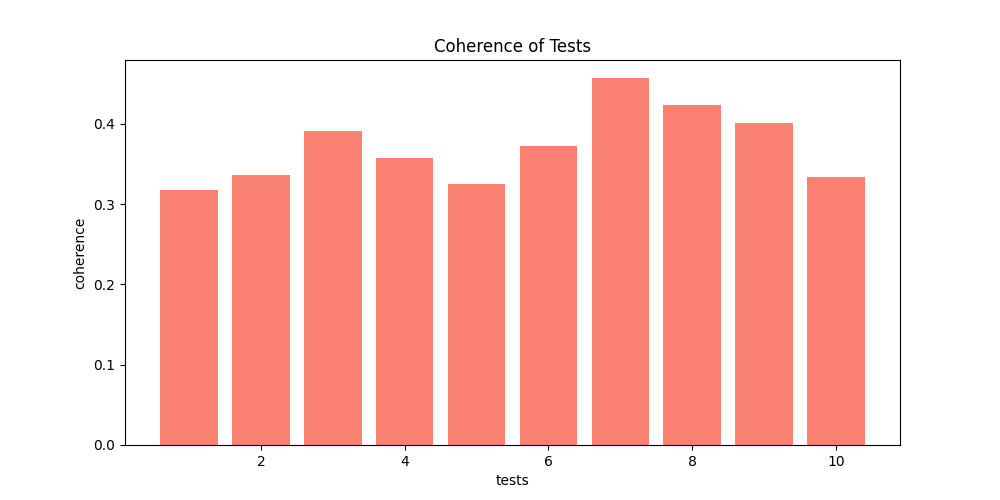
\includegraphics[width=7cm]{images/coherence_stopwords}
		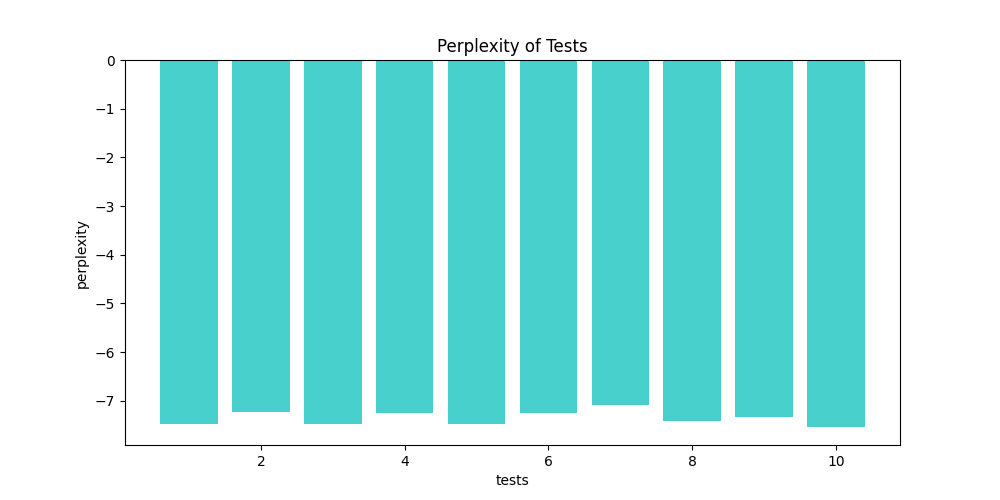
\includegraphics[width=7cm]{images/perplexity_stopwords}
	\caption{Coherence and perplexity values for each of the 50 tests with TokenVieuxM dataset.}
		\end{figure}
	
	The first thing we can notice is that different coherence and perplexity values are obtained in each run, even though we are working with the same corpus and number of topics. 
		
	In the LDA (\textit{Latent Dirichlet Allocation}) model, coherence and perplexity can vary when running the model multiple times with the same set of words. This can be attributed to various factors, such as random initialization of the model, parameter selection, quality of the training corpus, and the amount of available data. Additionally, different implementations of LDA may have variations in how coherence and perplexity are calculated, which can also contribute to differences in results. To address the issue of variability in coherence and perplexity in the LDA model of gensim when running it multiple times with the same set of words we can use a fixed random seed ensuring consistent initializations and obtaining more stable results. 
	
	The average values of perplexity and coherence across tests is approximately -7.33 and 0.38. 
	
	\subsection{Topic descriptions obtained with one specific launch}
	
	To further analyze the performance of the model let's look at the topic description obtained with one specific launch, in this case, test 5:

	\begin{figure}[H]
		\centering
		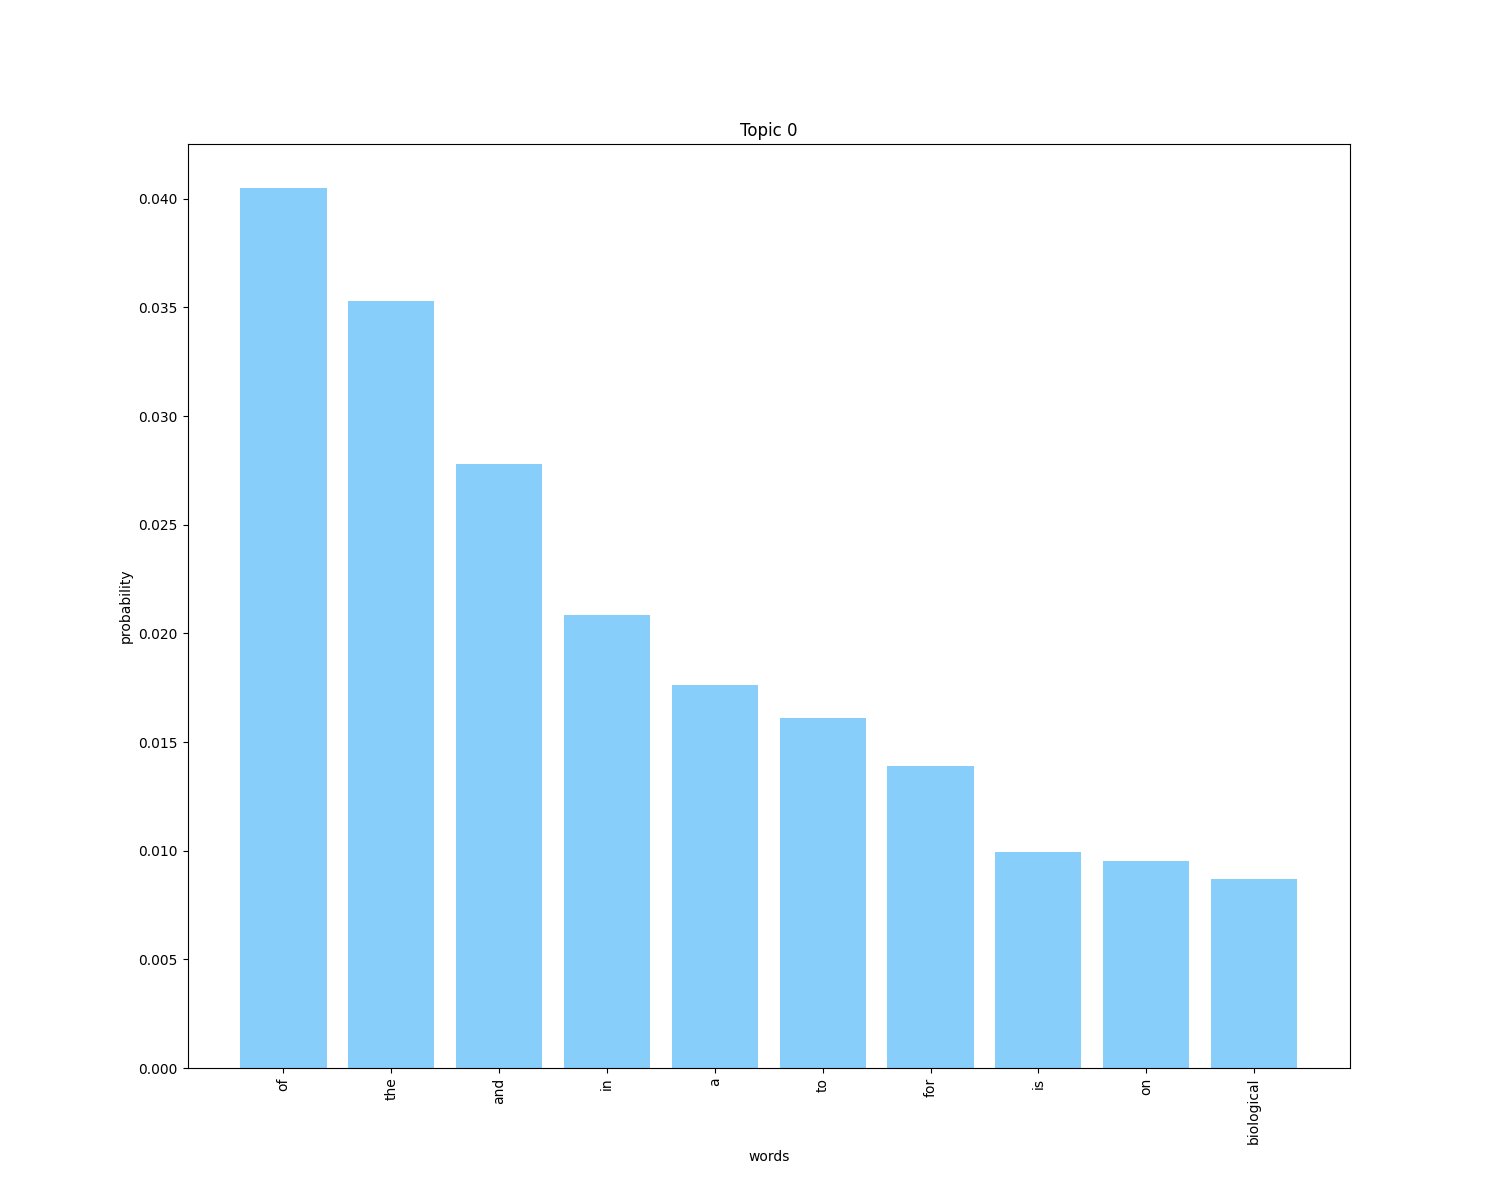
\includegraphics[width=7cm]{images/plots/test_5/topic_0.png}
		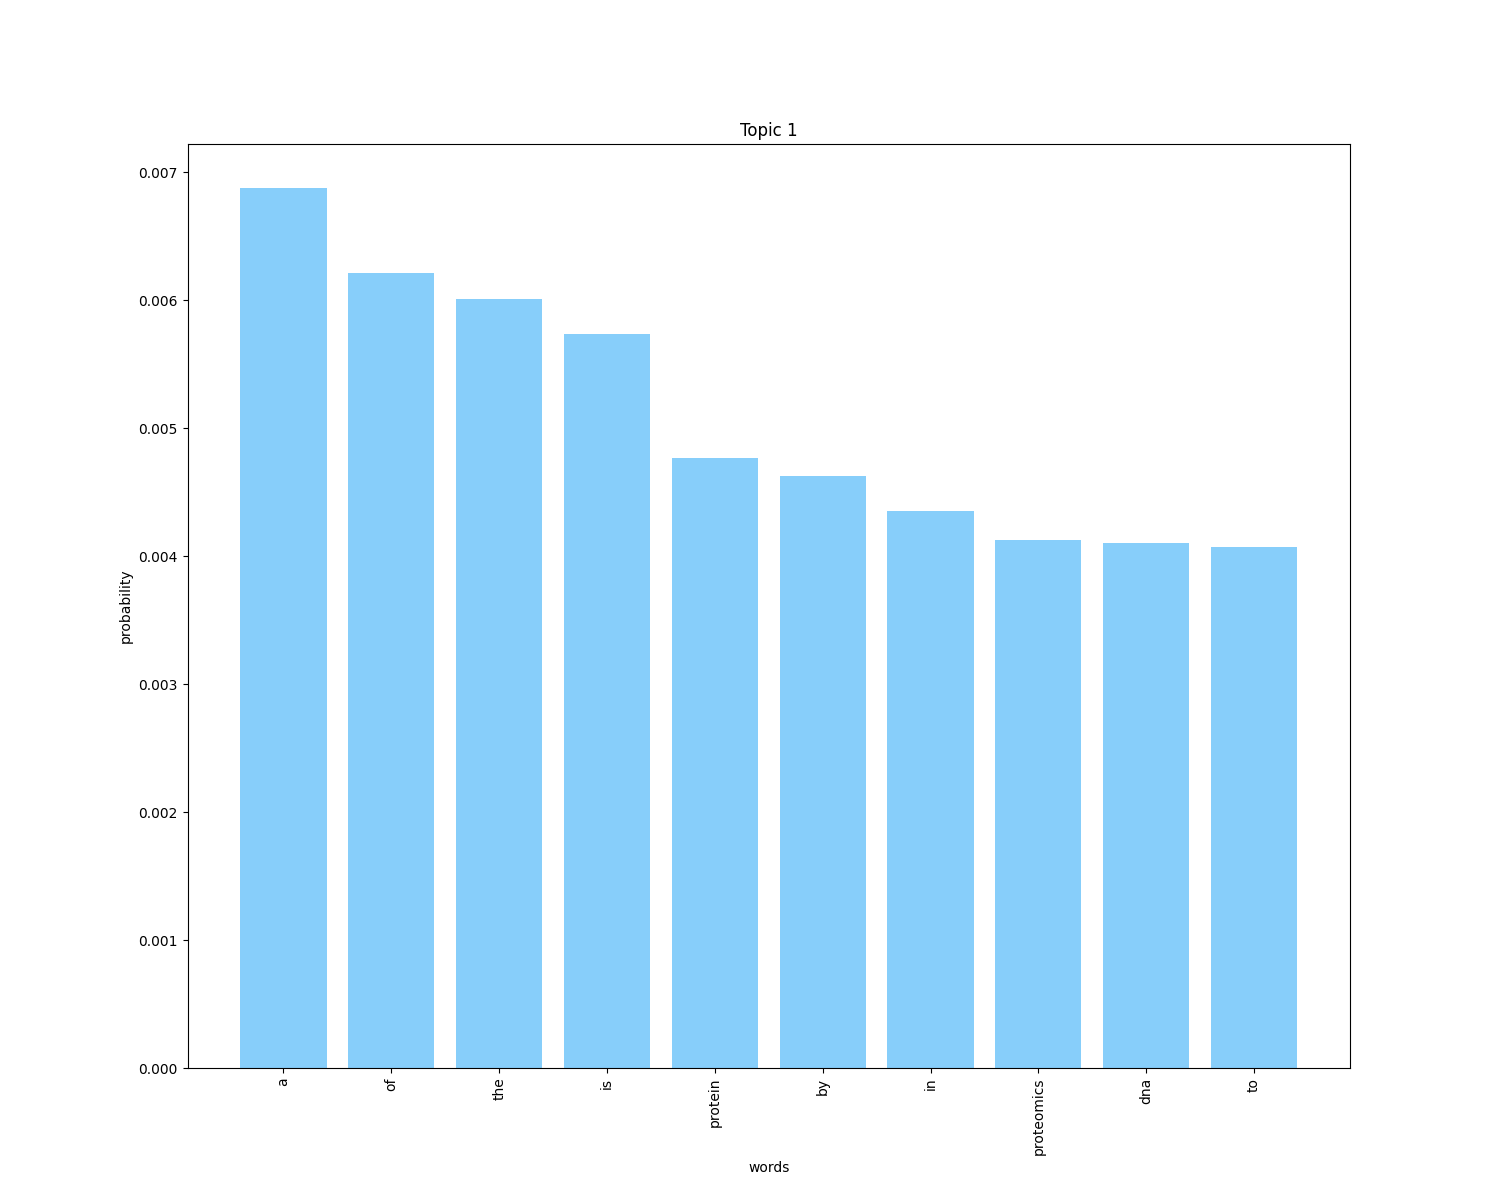
\includegraphics[width=7cm]{images/plots/test_5/topic_1.png}
	\end{figure}
	\begin{figure}[H]
		\centering
		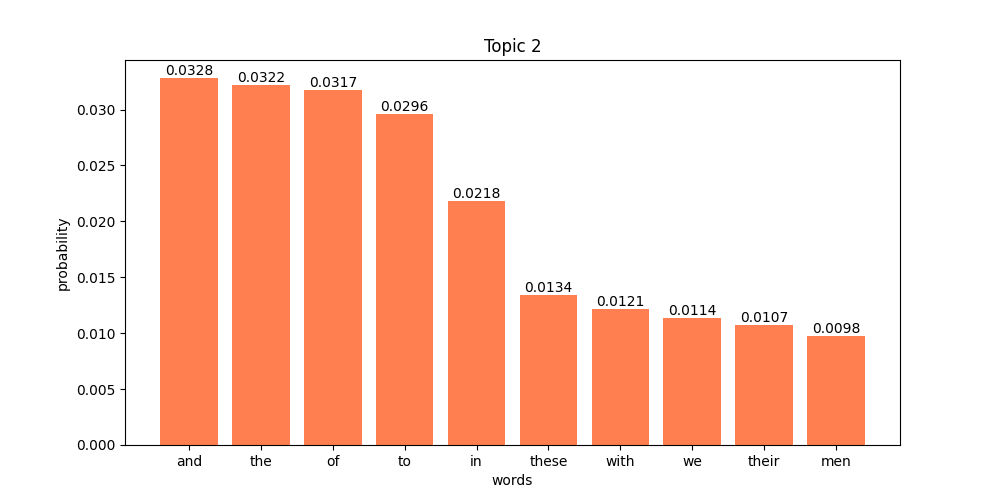
\includegraphics[width=7cm]{images/plots/test_5/topic_2.png}
		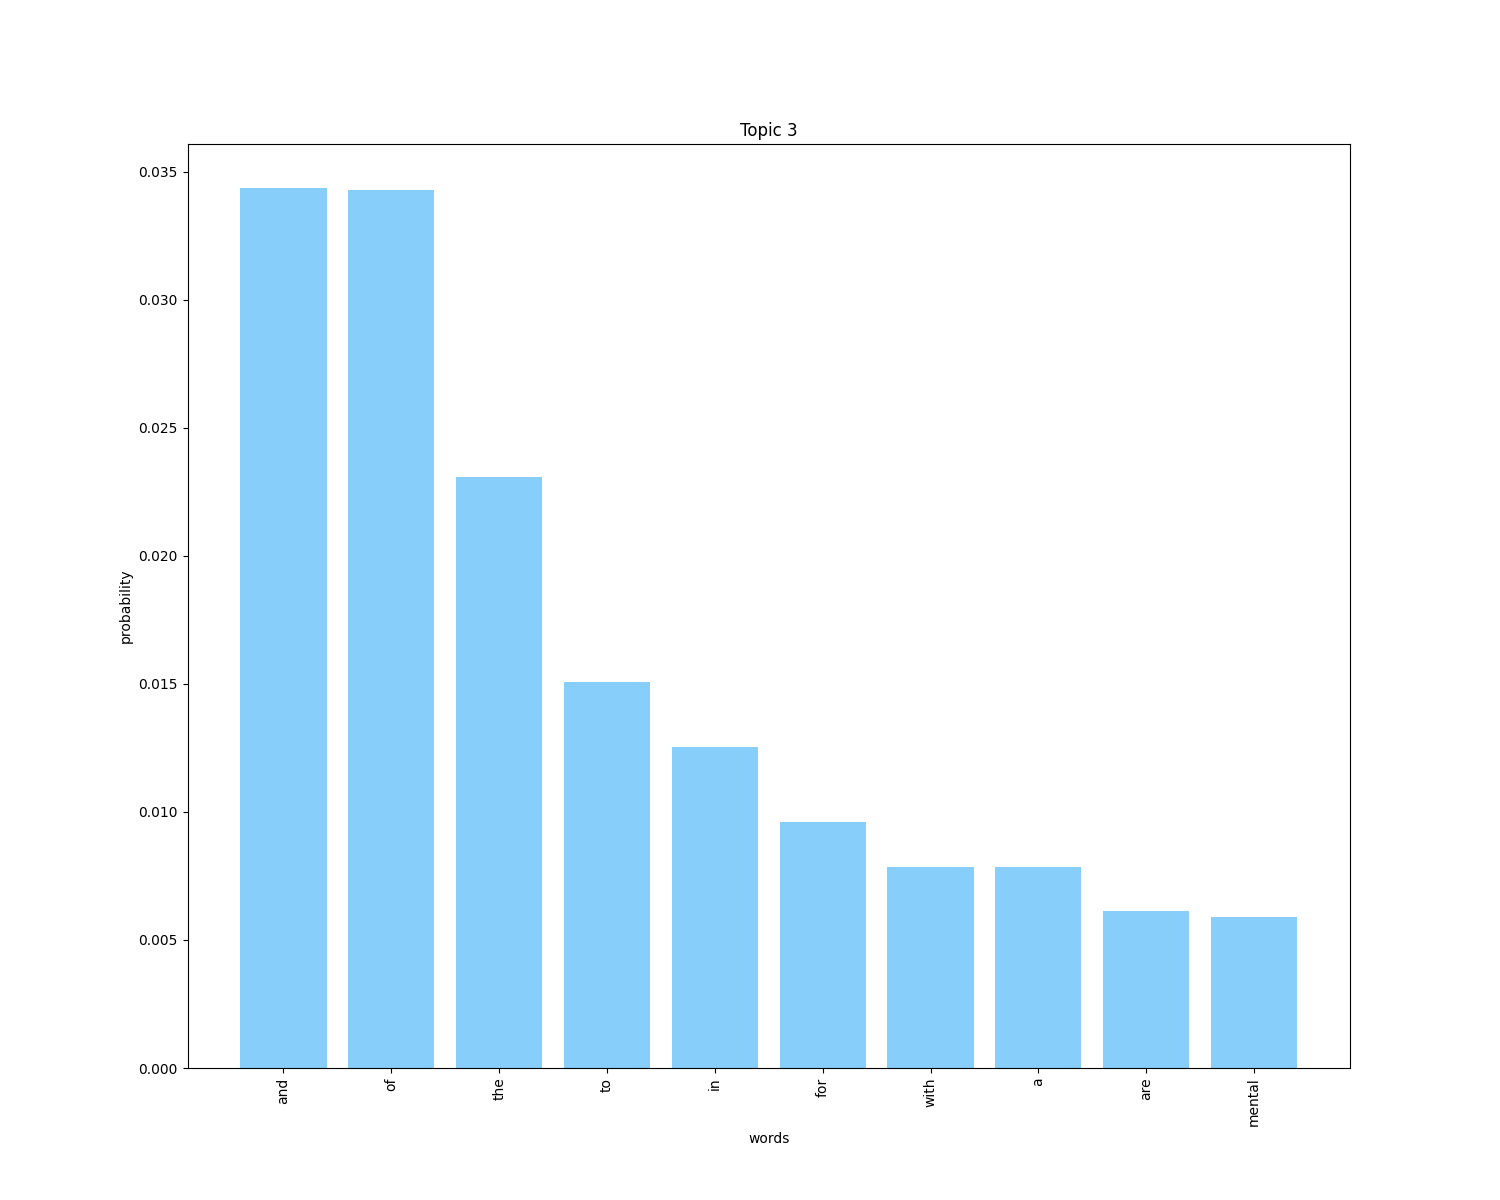
\includegraphics[width=7cm]{images/plots/test_5/topic_3.png}
		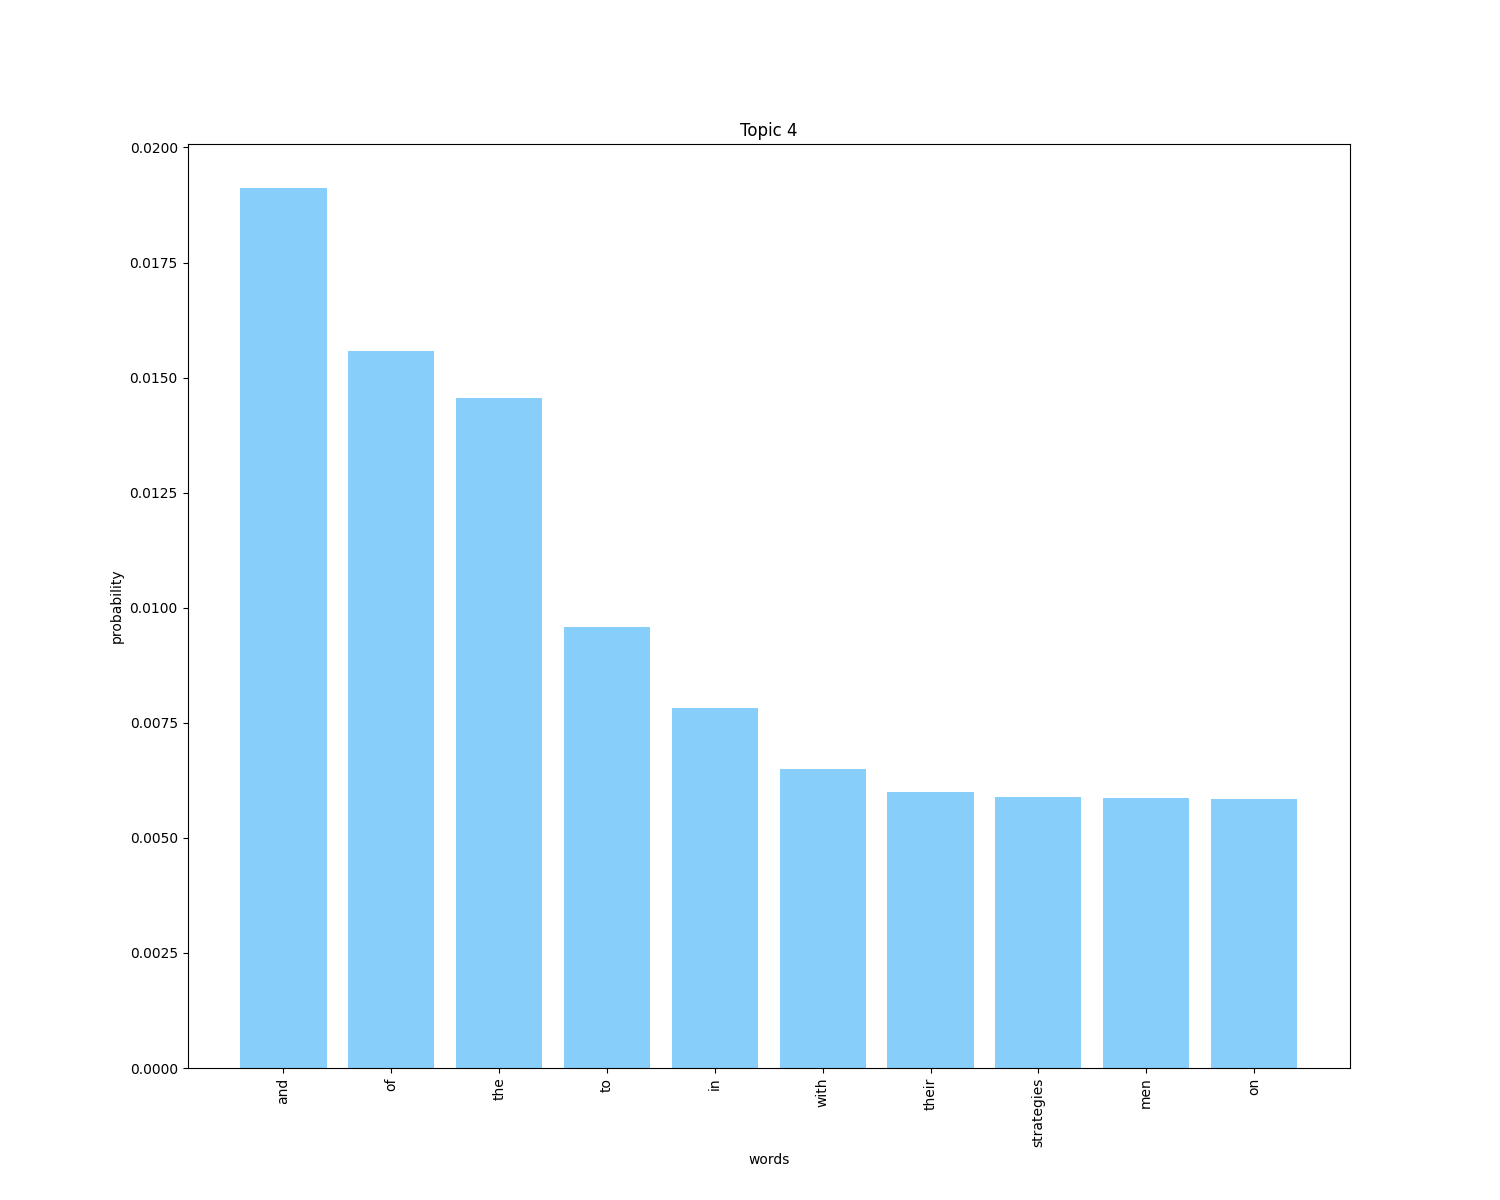
\includegraphics[width=7cm]{images/plots/test_5/topic_4.png}
		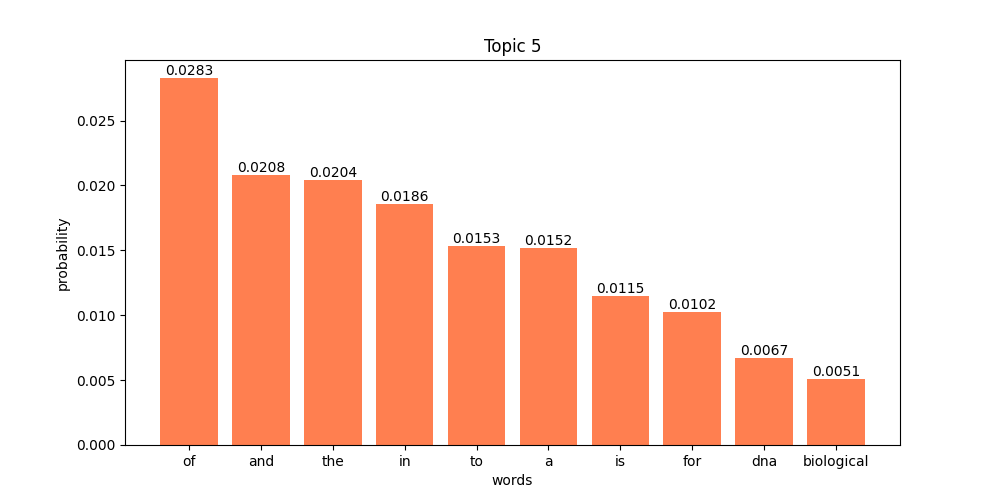
\includegraphics[width=7cm]{images/plots/test_5/topic_5.png}
		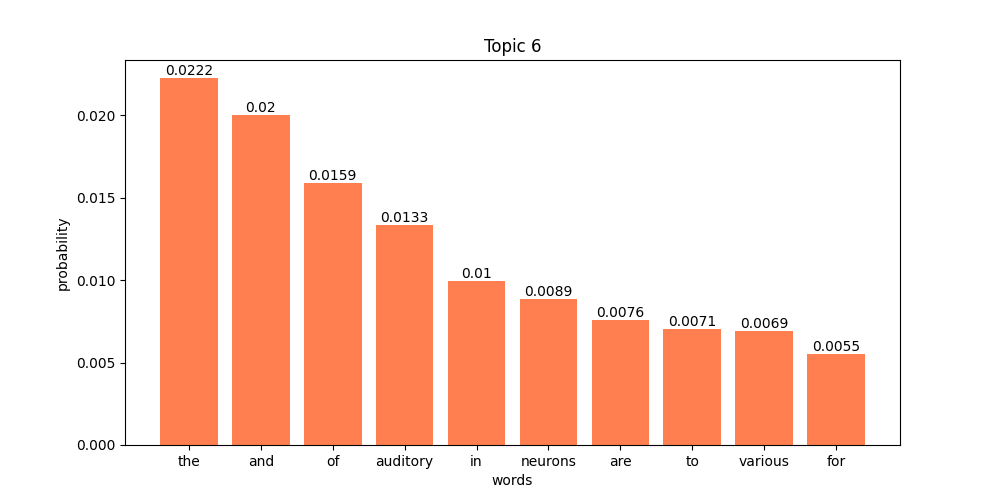
\includegraphics[width=7cm]{images/plots/test_5/topic_6.png}
		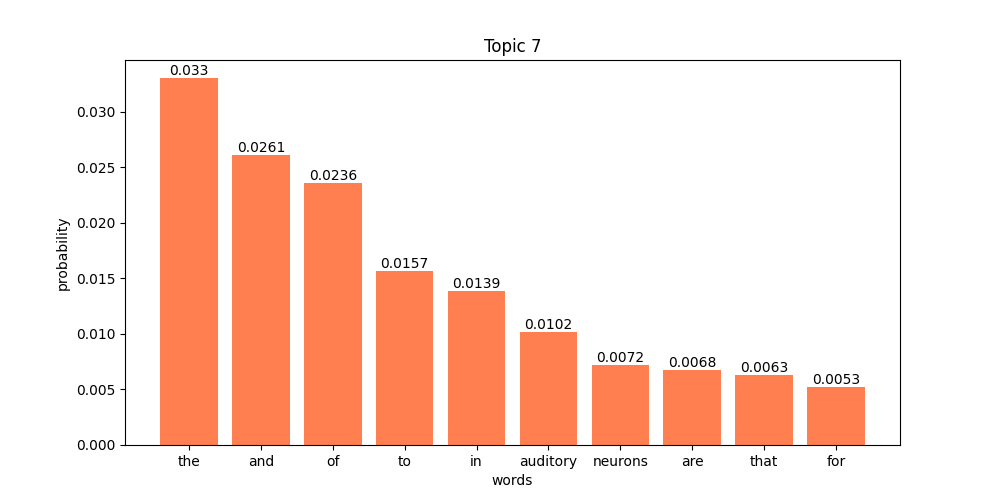
\includegraphics[width=7cm]{images/plots/test_5/topic_7.png}

	\caption{Topic description for test 5 of dataset TokenVieuxM.}
\end{figure}

	A significant issue was observed. The majority of the words that emerged in the topic descriptions were identified as stopwords. 

	\textit{Stopwords} are commonly used words in a language that are usually filtered out before or after processing of natural language data. Typically they consist in articles, prepositions, conjunctions, or pronouns. Examples of stopwords in English include "a", "the", "is", "are", and so on. The presence of these stopwords in the topic descriptions is problematic because they appear in almost every document. They are generally uninformative in the context of an LDA model, as they do not contribute to the theme or subject of a topic. The high prevalence of stopwords in the topic descriptions makes it challenging to interpret the topics and understand the underlying themes in the dataset.
	
	In terms of the model's performance metrics, the coherence value is relatively low, 0.40, which is consistent with the observation that the topics are difficult to interpret due to the high presence of stopwords. The perplexity value was -7.33 which does not provide a clear indication of the model's performance. 
	
	\section{Removing stopwords}
	
	The removal of stopwords in the Latent Dirichlet Allocation (LDA) model indeed plays a crucial role in enhancing the quality of the topics generated. By eliminating these common words, which typically do not contribute to the meaning or theme of a topic, the model can focus on the most significant words for topic identification. This not only improves the interpretability of the topics but also reduces the dimensionality of the word space used, making the model more efficient.
	
	A new Python script was created in which the lines of code responsible for removing stopwords from the given set of words in TokenVieuxM.txt were uncommented. This modification is expected to improve the performance of the model. 
	
		\begin{figure}[H]
		\centering
		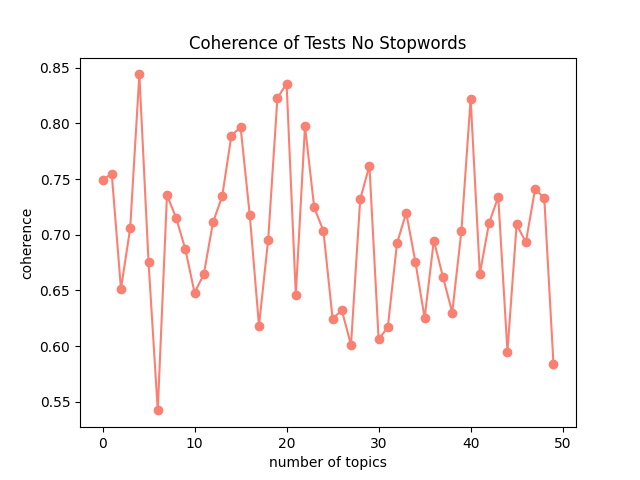
\includegraphics[width=7cm]{images/coherence_no_stopwords}
		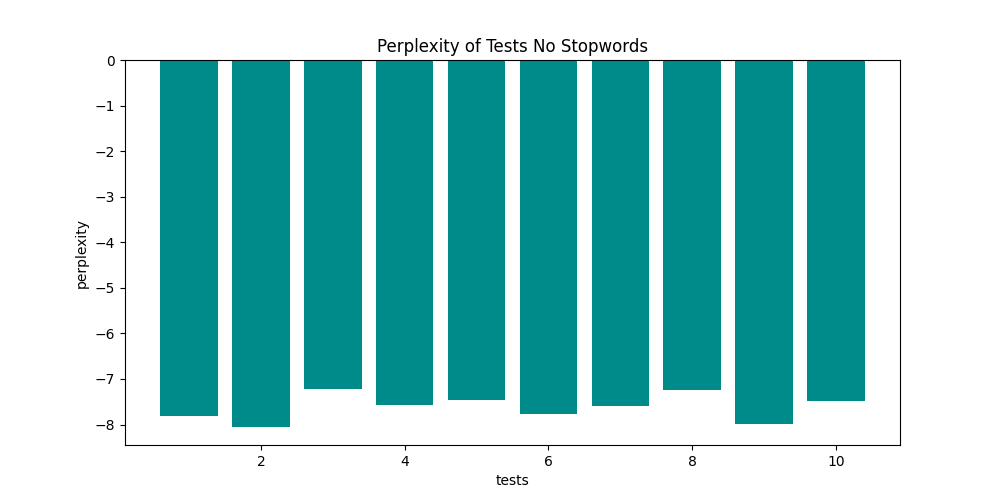
\includegraphics[width=7cm]{images/perplexity_no_stopwords}
	\caption{Coherence and perplexity values for each of the 50 tests with TokenVieuxM dataset after removing stopwords.}
\end{figure}
	
	The average values of perplexity and coherence across tests is approximately -7.78 and 0.70. 
	
	\subsection{Topic descriptions obtained with one specific launch and no stopwords}\label{test_8_ns_1}
	
	Once again, let's look at the topic description obtained with one specific launch of test 5:
	
		\begin{figure}[H]
		\centering
		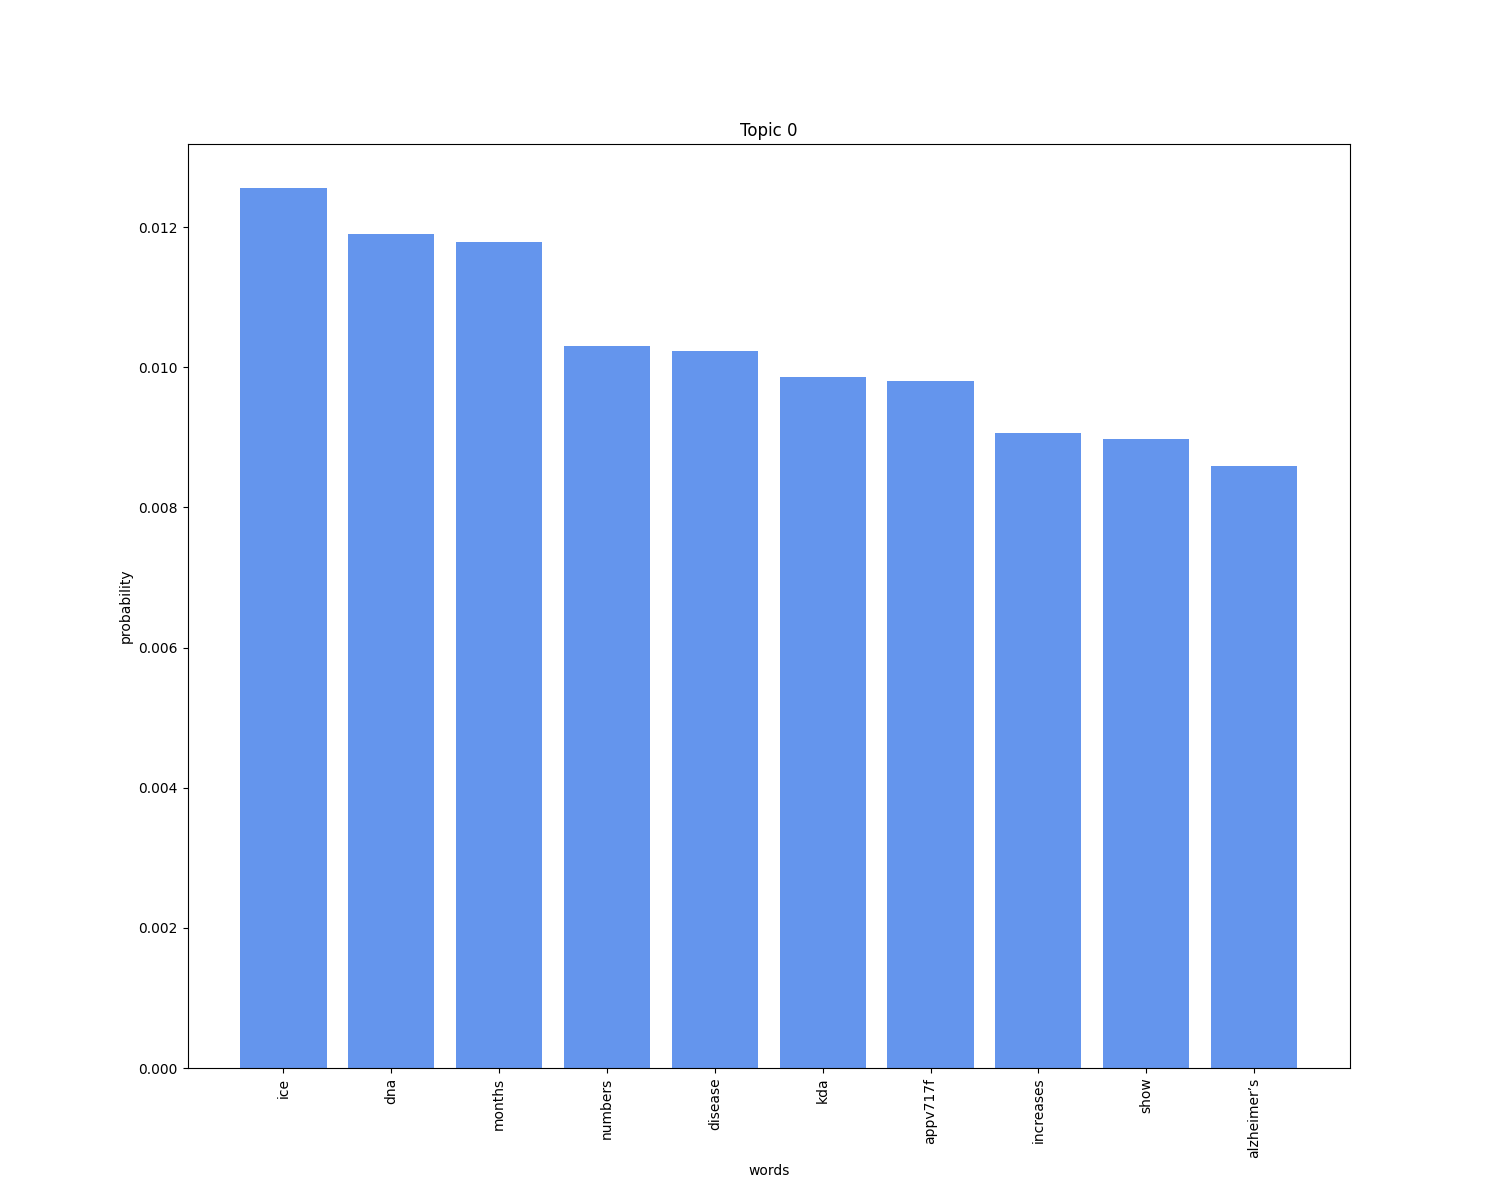
\includegraphics[width=7cm]{images/plots/test_5_no_stopwords/topic_0.png}
		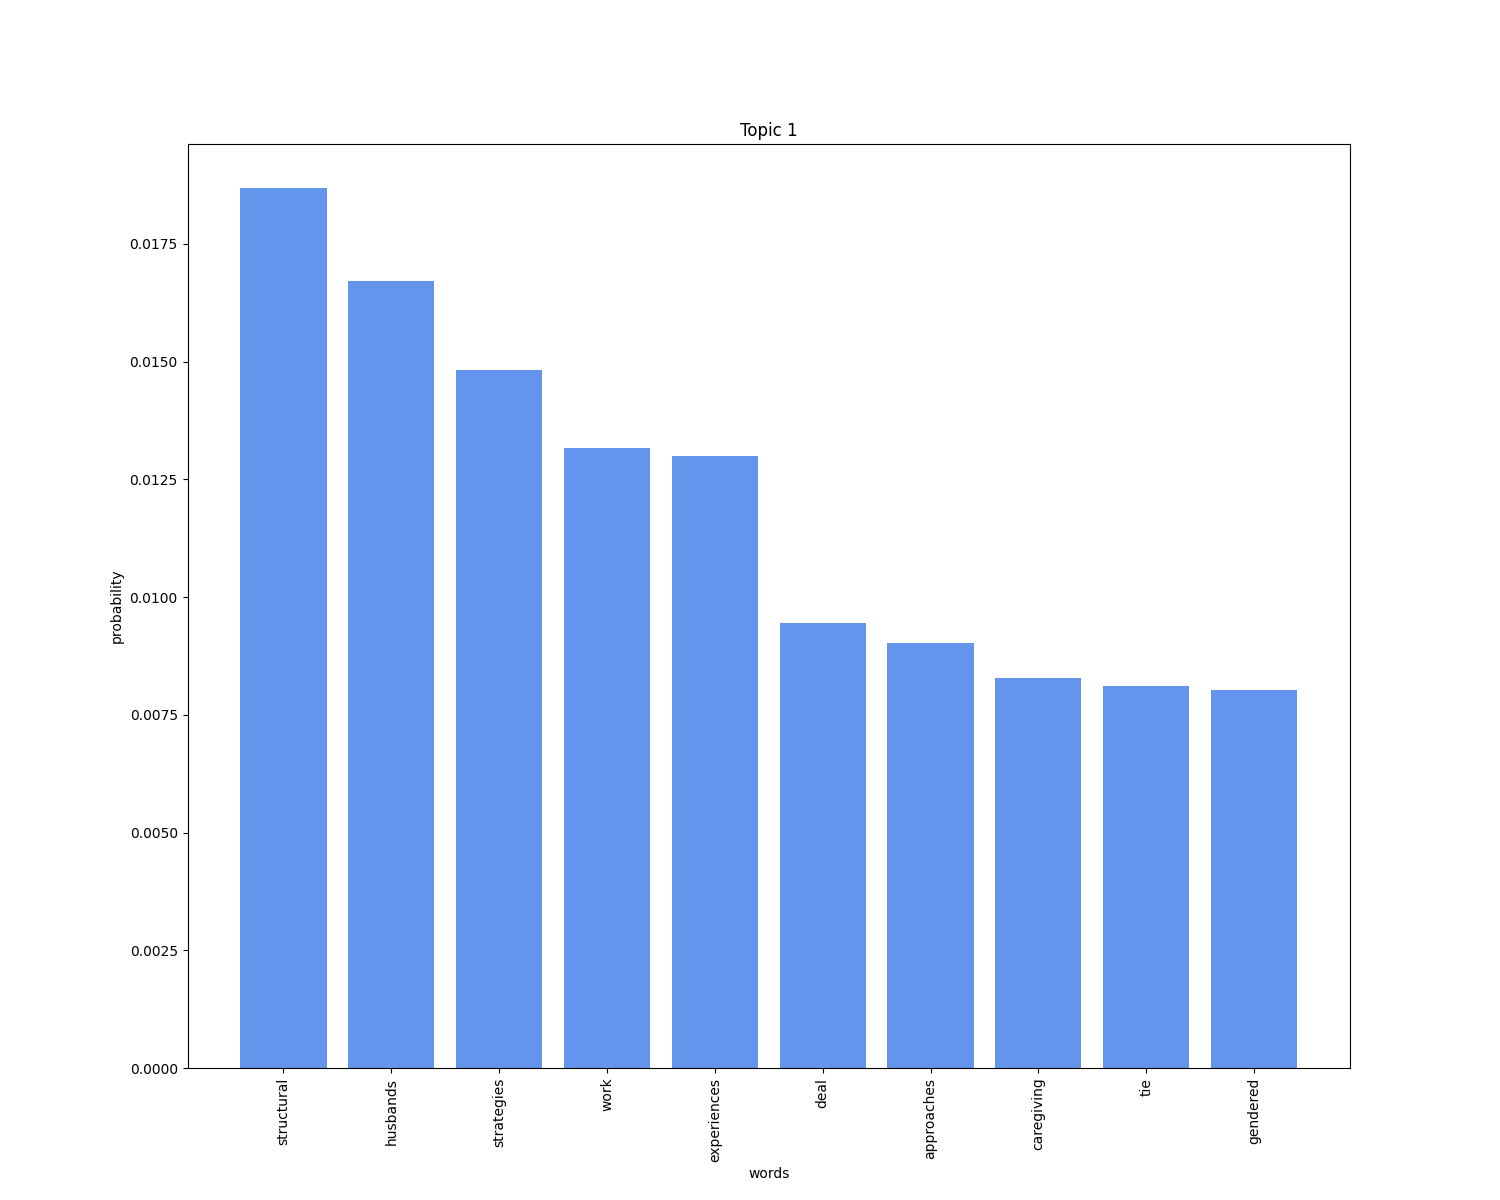
\includegraphics[width=7cm]{images/plots/test_5_no_stopwords/topic_1.png}
		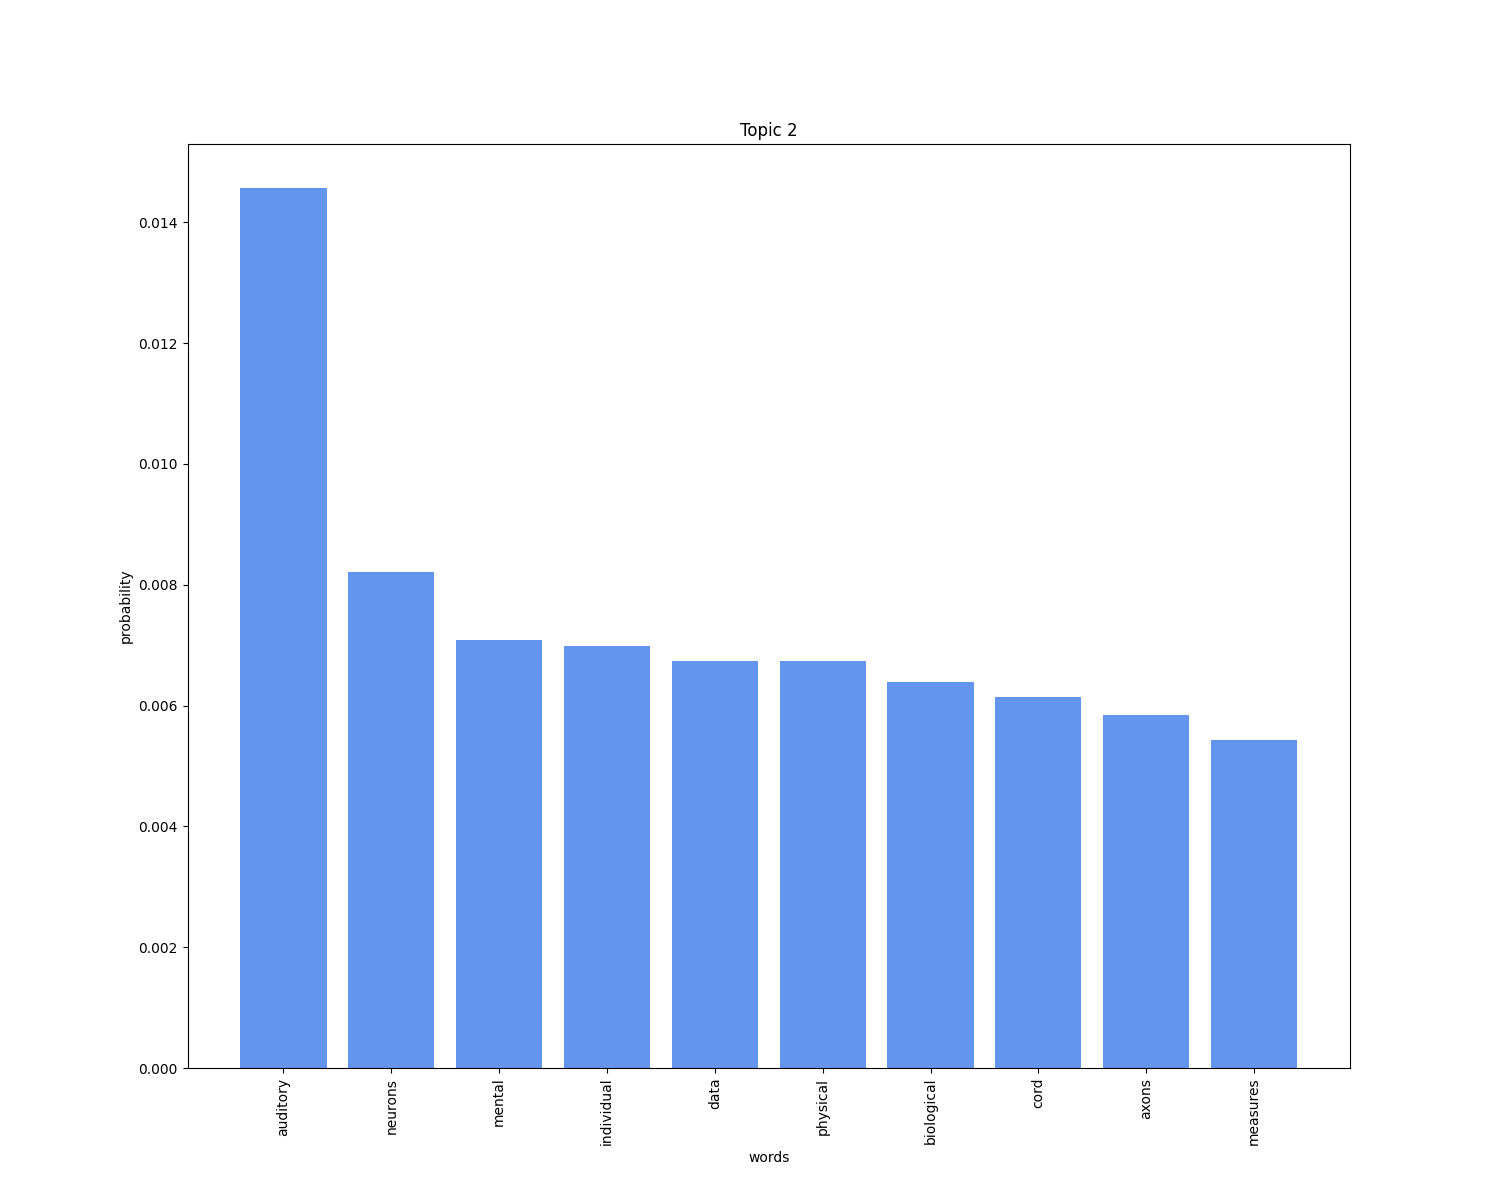
\includegraphics[width=7cm]{images/plots/test_5_no_stopwords/topic_2.png}
		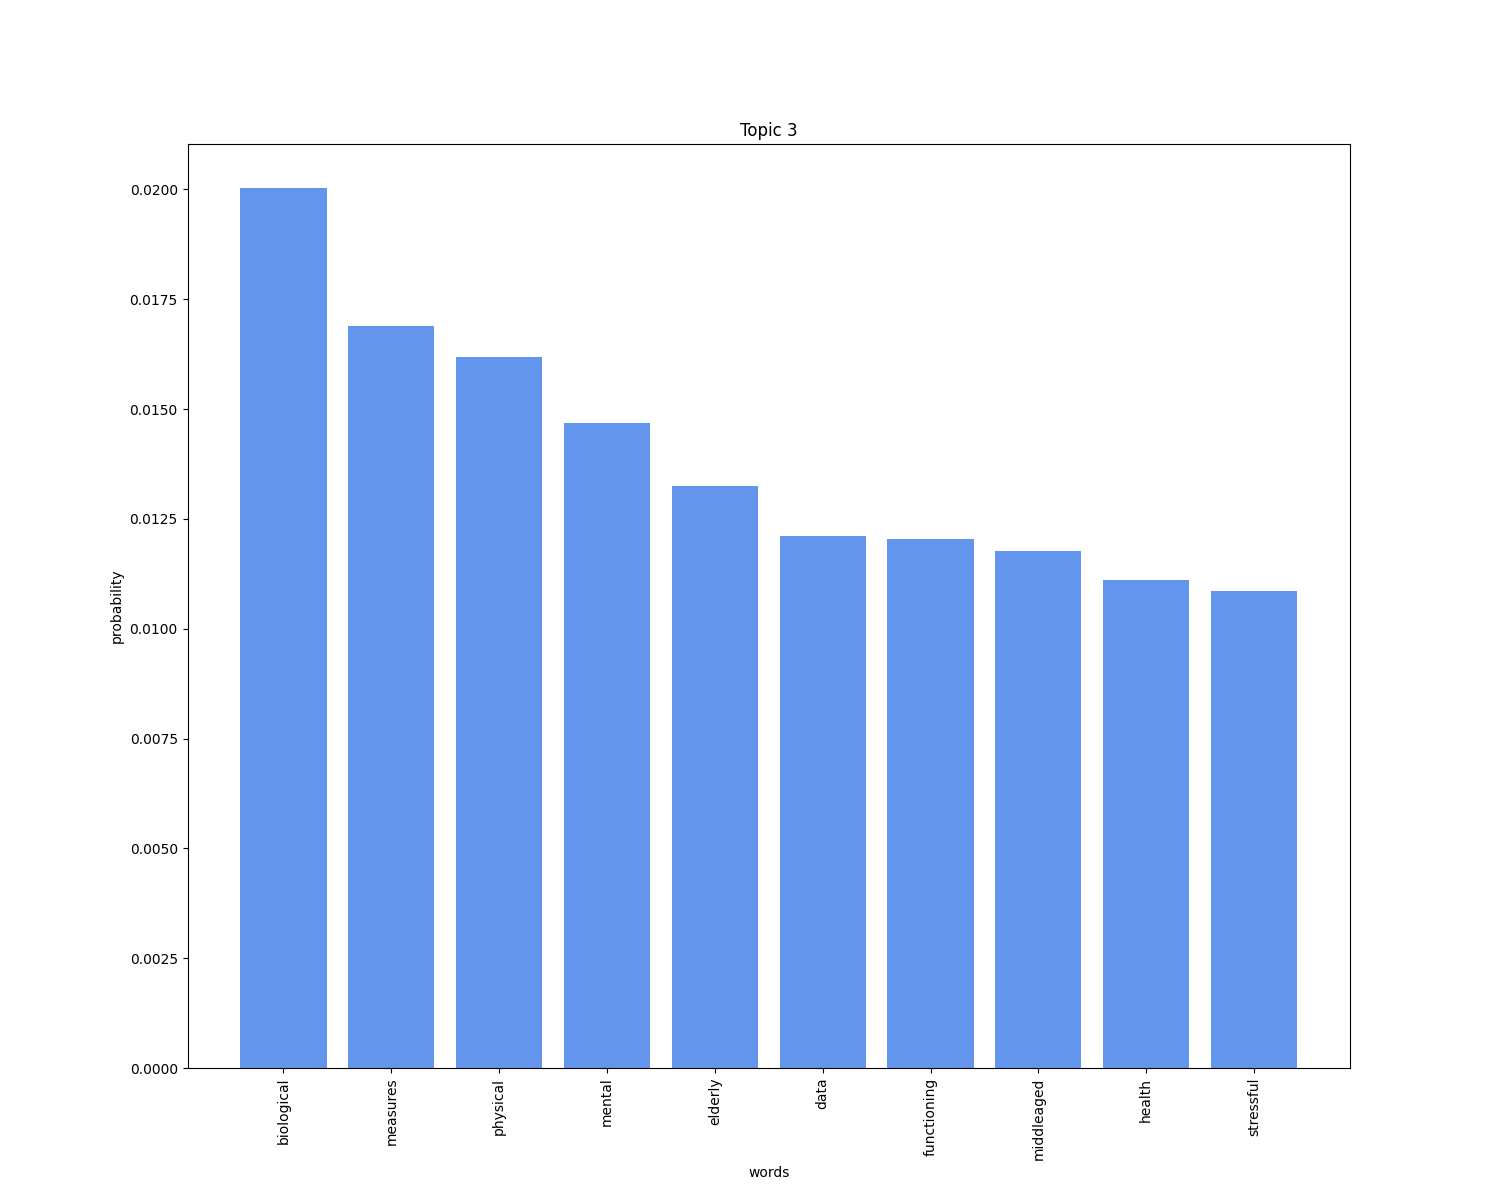
\includegraphics[width=7cm]{images/plots/test_5_no_stopwords/topic_3.png}\
		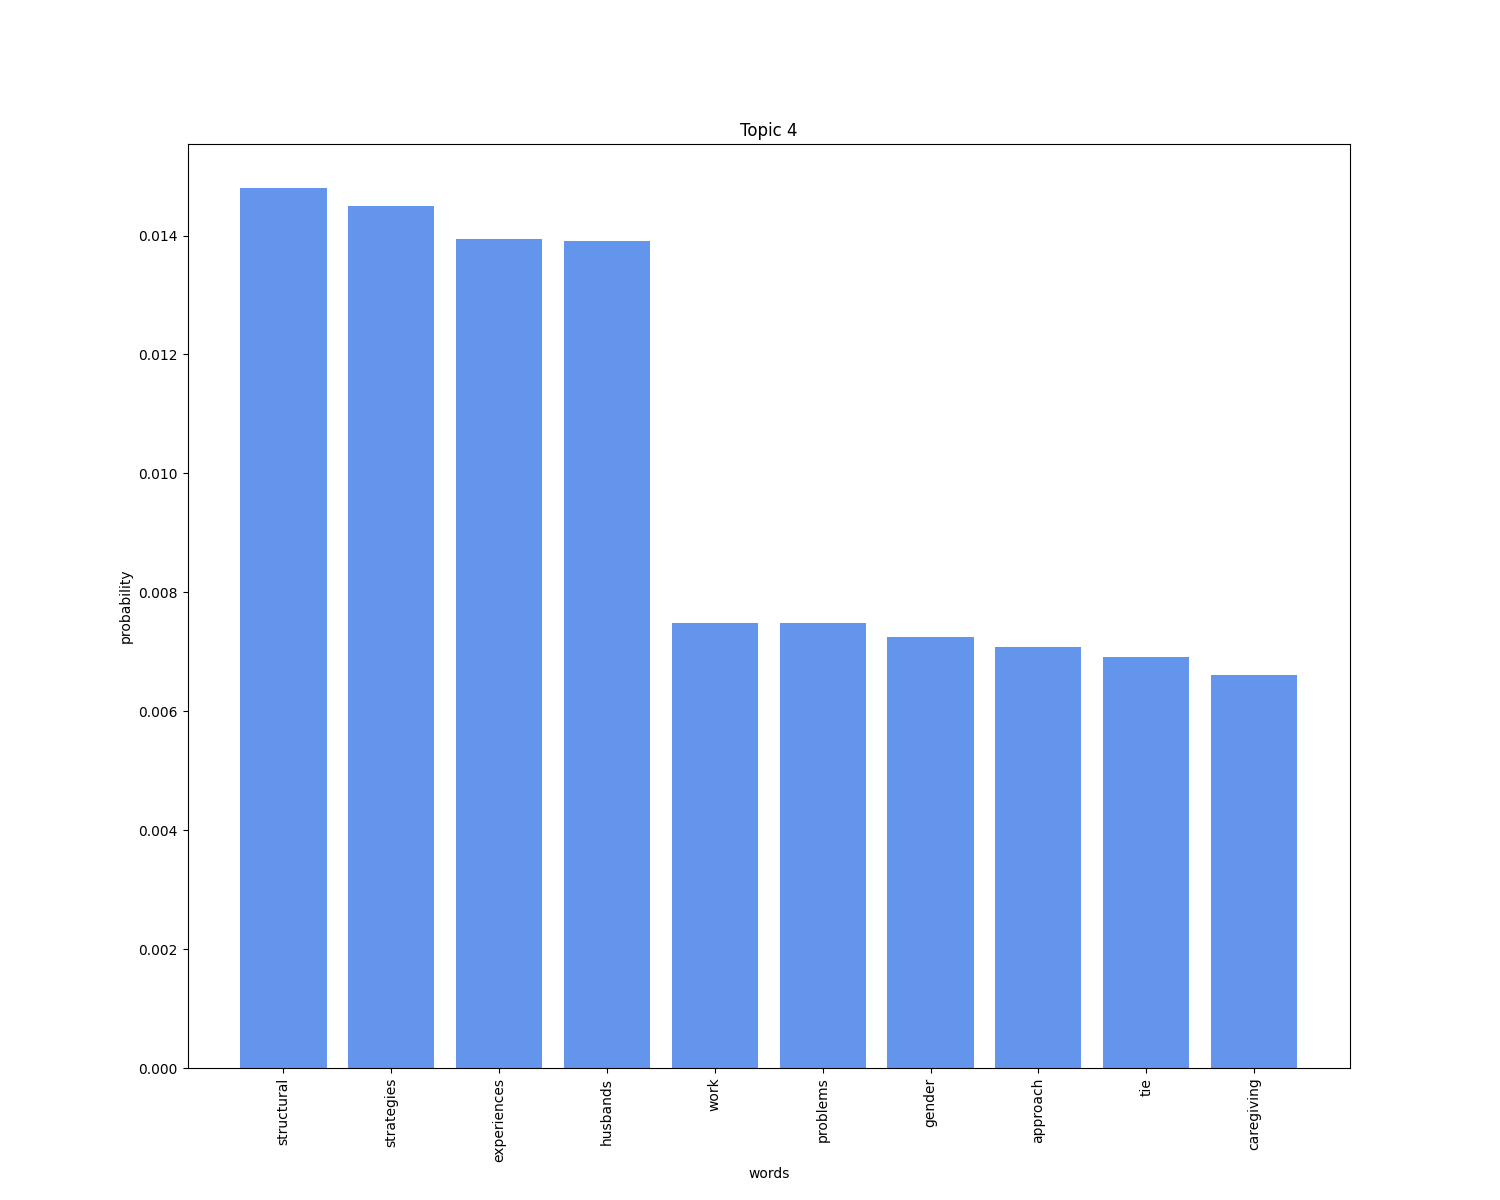
\includegraphics[width=7cm]{images/plots/test_5_no_stopwords/topic_4.png}
		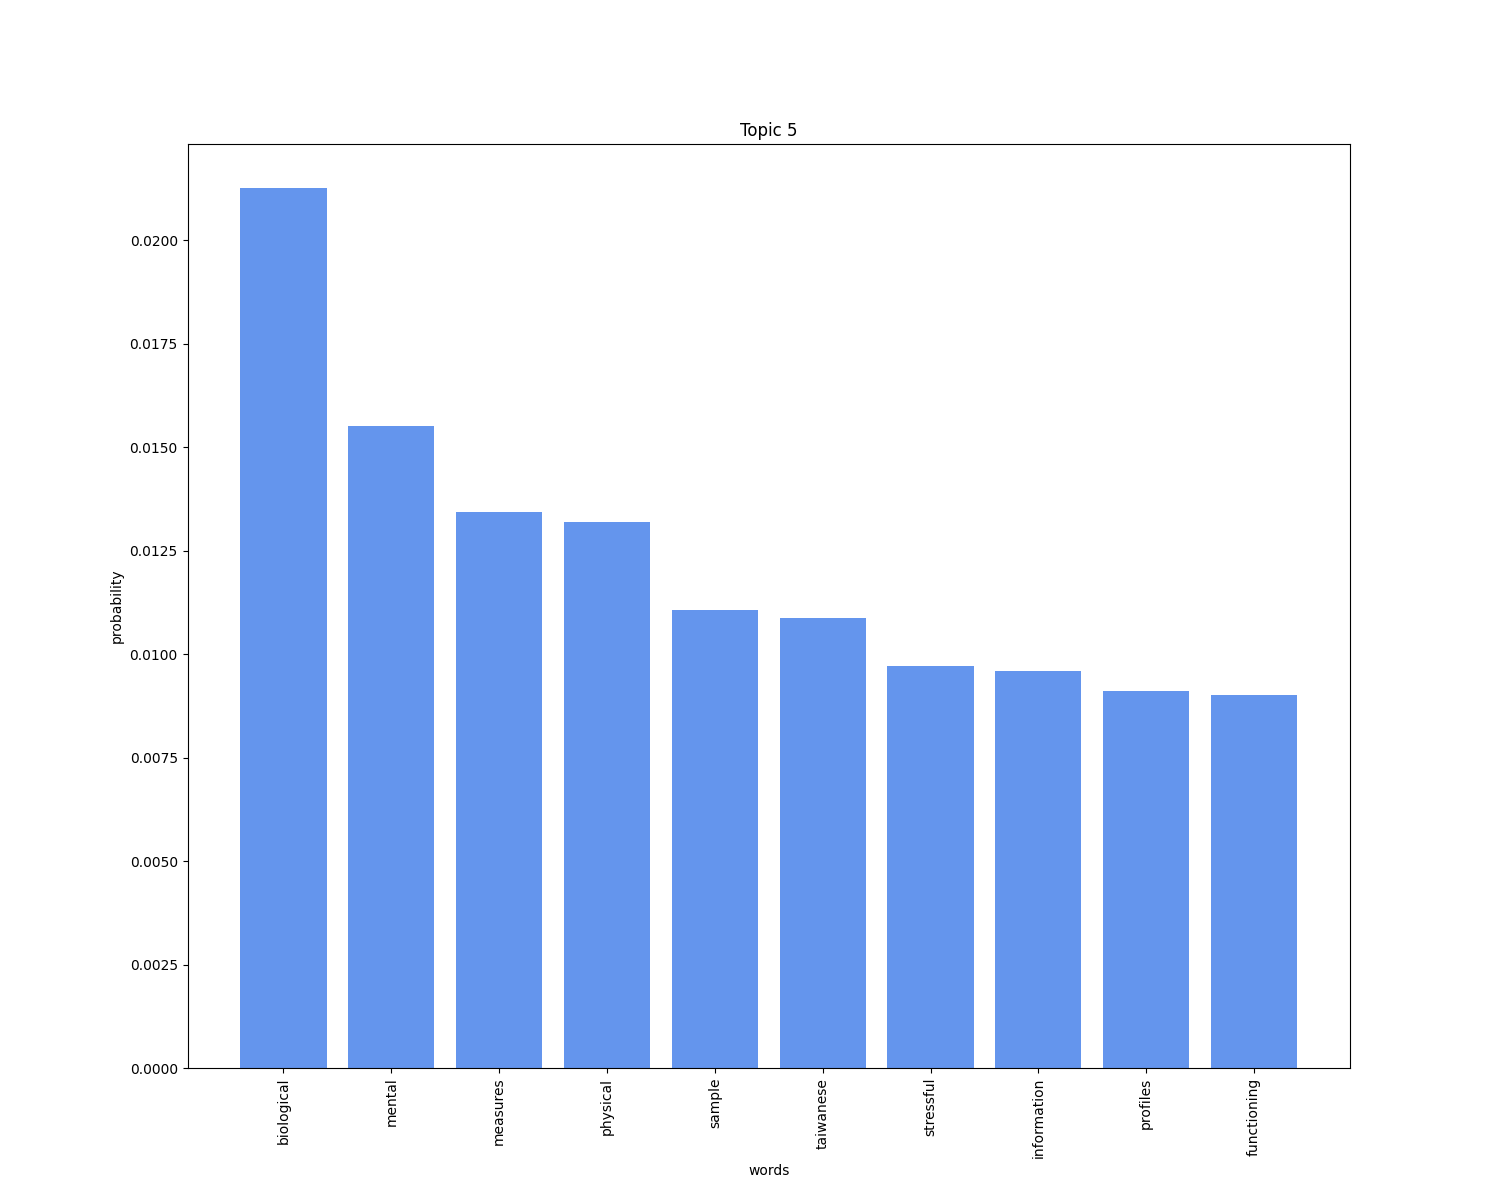
\includegraphics[width=7cm]{images/plots/test_5_no_stopwords/topic_5.png}
		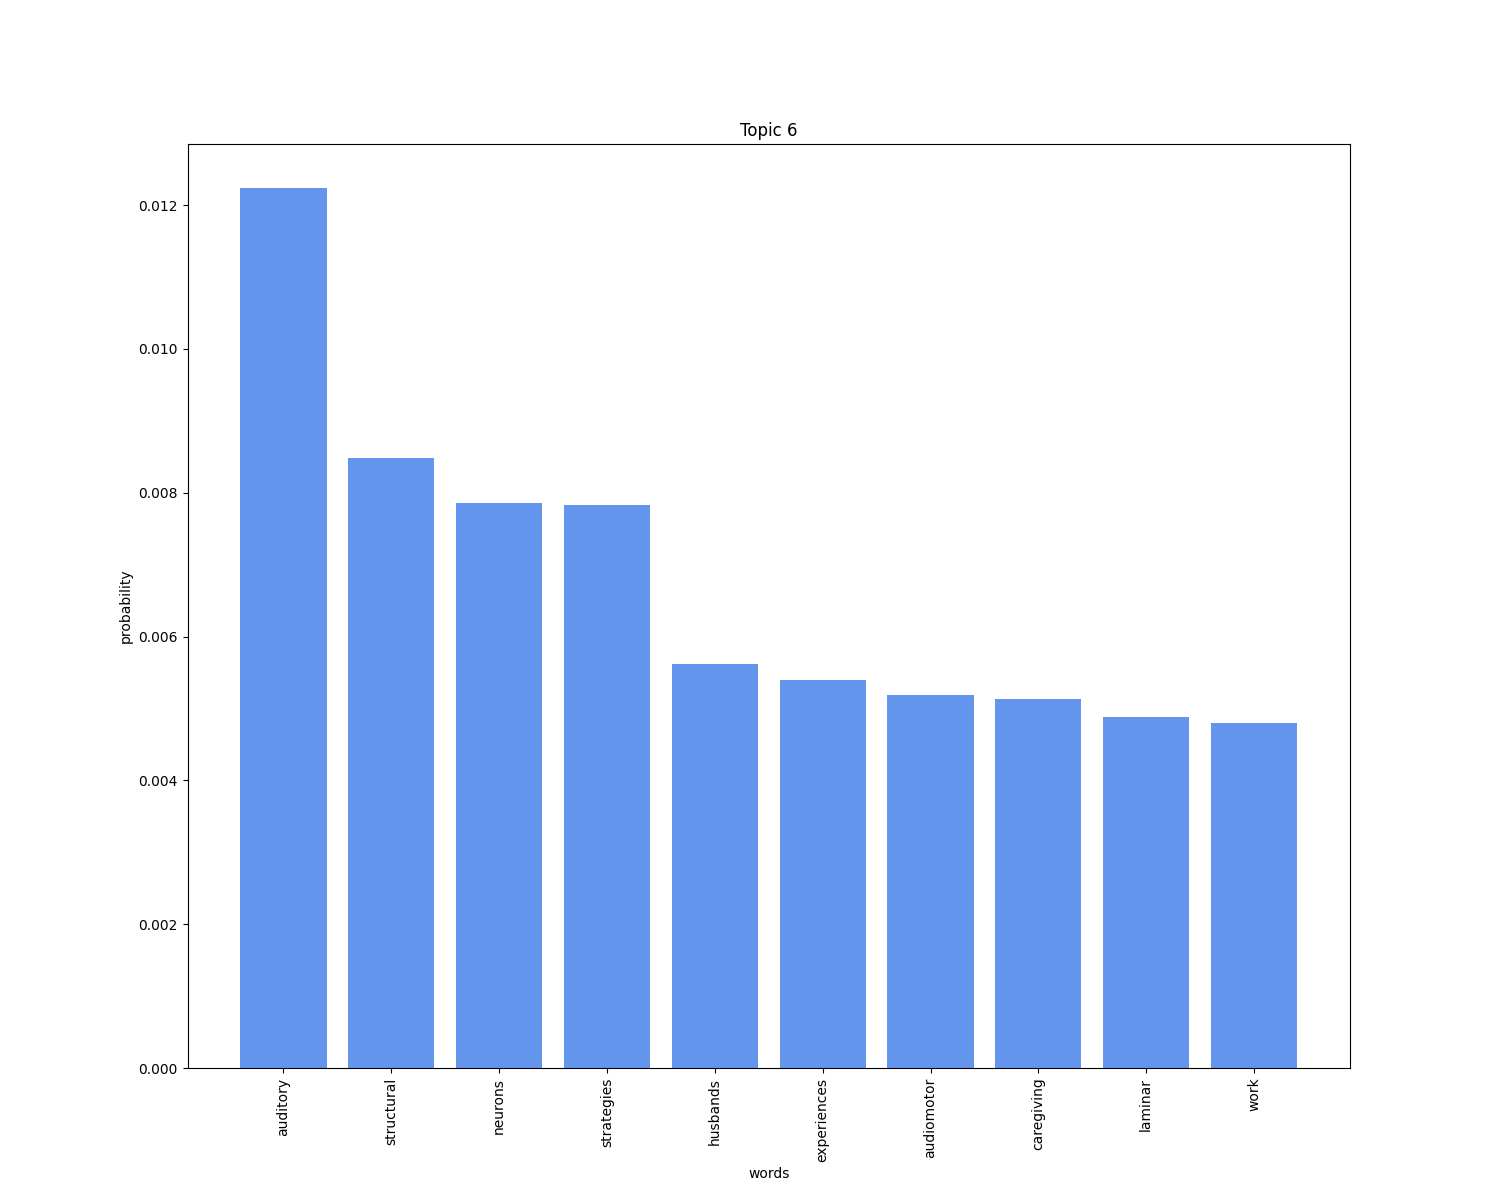
\includegraphics[width=7cm]{images/plots/test_5_no_stopwords/topic_6.png}
		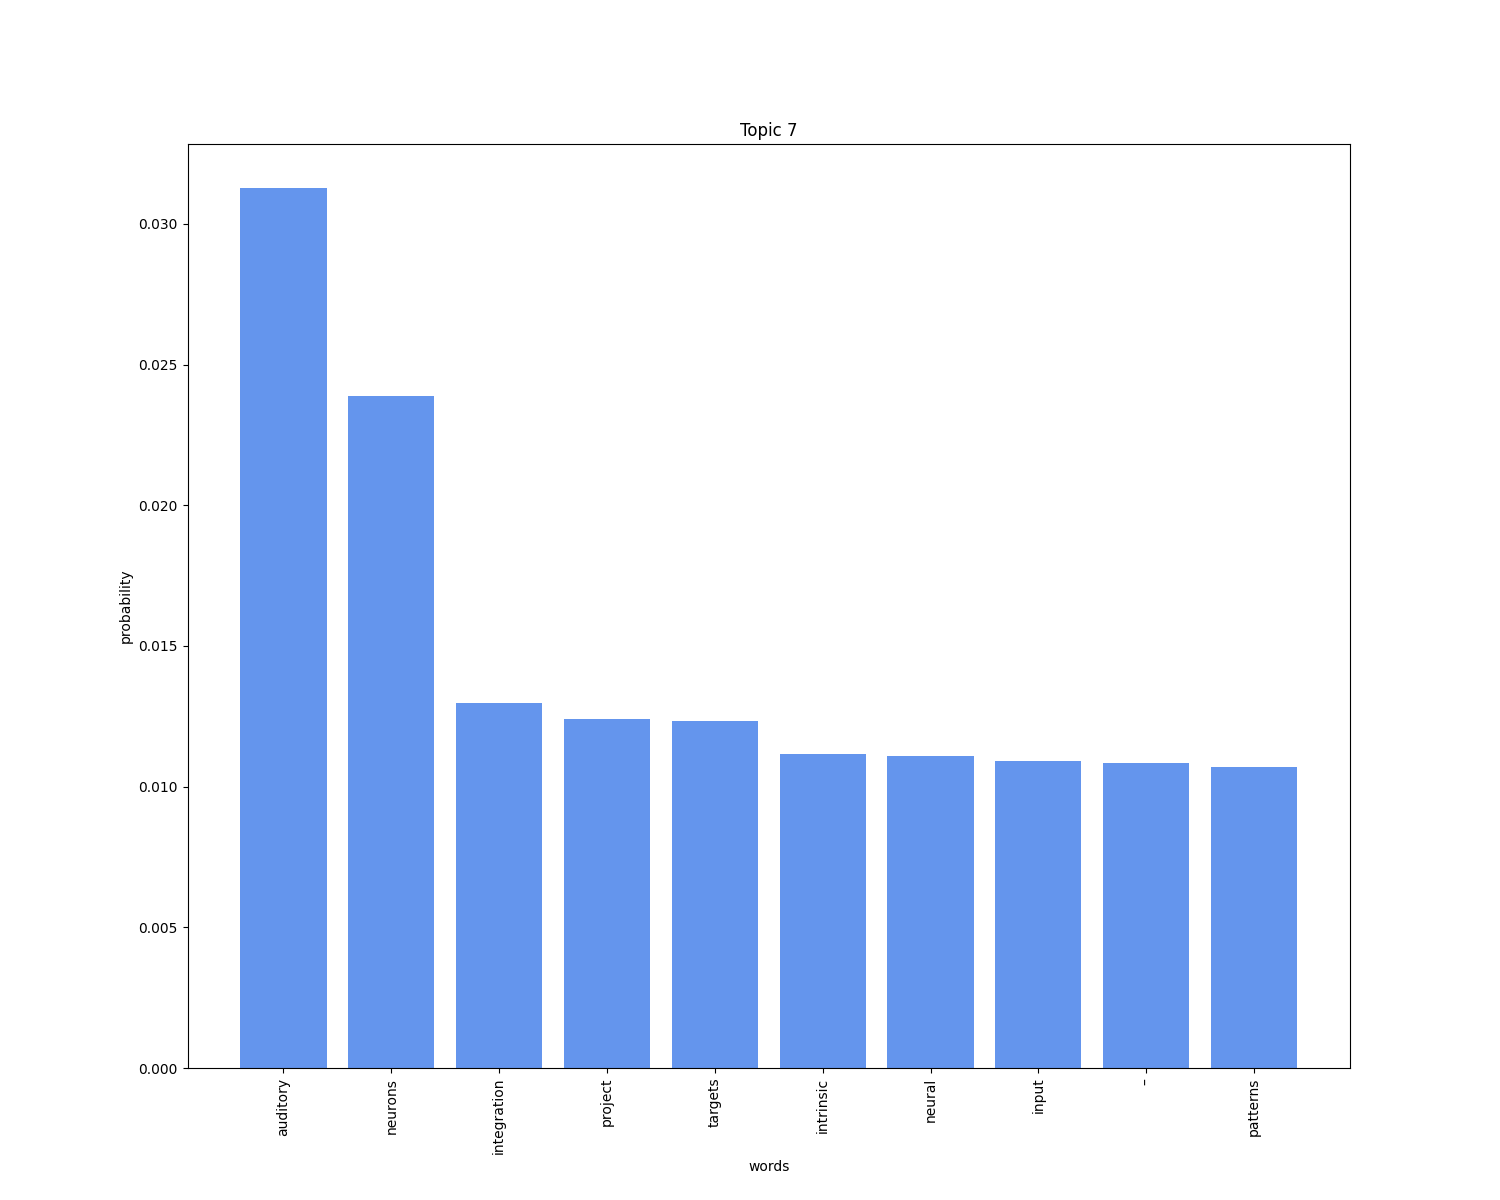
\includegraphics[width=7cm]{images/plots/test_5_no_stopwords/topic_7.png}
	\caption{Topic description for test 5 of dataset TokenVieuxM after removing stopwords.}
\end{figure}
	
	In this case a slightly lower perplexity was obtained, -7.72 while the coherence increased to 0.66. These changes suggest that the removal of stopwords from the dataset improved the performance of the LDA model, both in terms of its predictive ability (as indicated by the decrease in perplexity) and the interpretability of its topics (as indicated by the increase in coherence). This underscores the importance of preprocessing steps in natural language processing tasks.
	
	\section{Optimal number of topics for the document collection TokenVieuxM.txt}
	
	Choosing the optimal number of topics in an LDA model is a crucial step, but there isn't a definitive rule for this as it largely depends on the specific dataset and the context of the problem. 
	
	\begin{figure}[H]
	\centering
		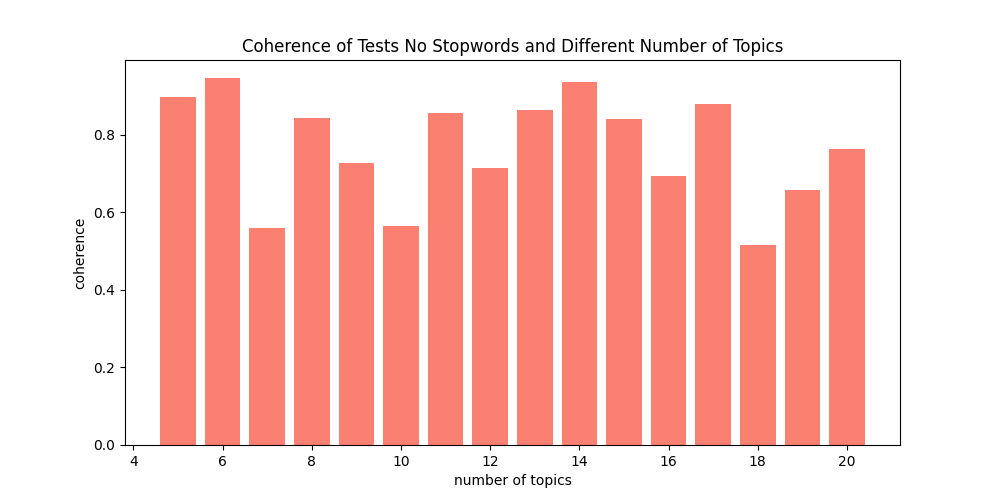
\includegraphics[width=7cm]{images/coherence_no_stopwords_diff_n_topics}
		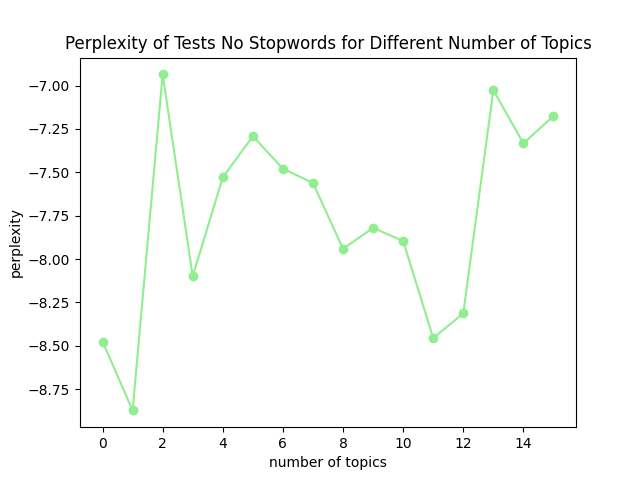
\includegraphics[width=7cm]{images/perplexity_no_stopwords_diff_n_topics}
	\caption{Coherence and perplexity values of the model for each number of topic $k \in [5, 20]$ , in dataset TokenVieuxM.}
\end{figure}
	
	In the process of determining the optimal number of topics for the LDA model, it is generally accepted that a model with lower perplexity and higher coherence is more desirable. A technique often used is the elbow method, as in K-Means. However, in the absence of a discernible elbow in the plot of these metrics, a different approach is required.
	
	We propose to make this decision by computing the difference between the coherence and perplexity values for each model. This difference will serve as a composite metric that balances both the predictive accuracy (as indicated by perplexity) and interpretability (as indicated by coherence) of the model. Among the models evaluated, we will select the one with the highest value of this composite metric. However, in cases where multiple models have similar composite scores, we will prioritize the model with the higher coherence value. This is due to our specific need for easily interpretable topics, which is better facilitated by a higher coherence score. This approach ensures that we select a model that not only fits the data well but also generates topics that are semantically meaningful and interpretable.
	
	According to this strategy, the optimal number of topics would be 5.
	
	\section{Changing the dataset}
	
	Let us now analyze the behavior of the model for the document collection TokenVieuxN.txt. The program was also executed 50 times, and the following coherence and perplexity values were obtained:
	
	\begin{figure}[H]
	\centering
		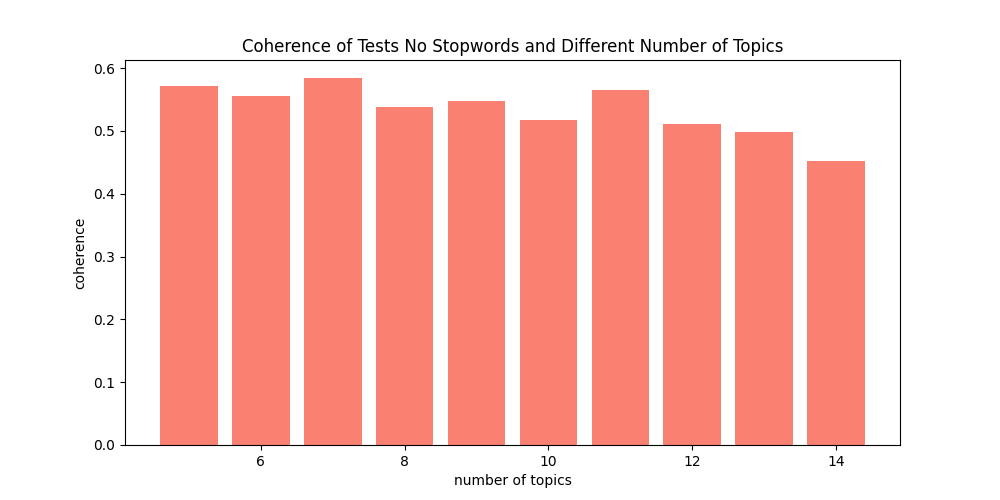
\includegraphics[width=7cm]{images/coherence_no_stopwords_2}
		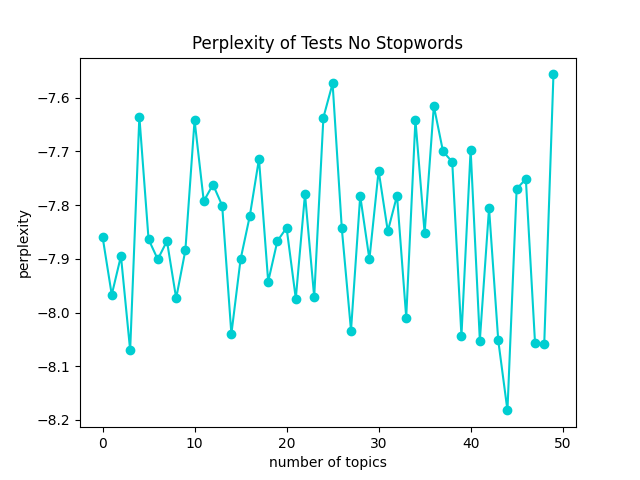
\includegraphics[width=7cm]{images/perplexity_no_stopwords_2}
	\caption{Coherence and perplexity values for each of the 50 tests with TokenVieuxN dataset after removing stopwords.}
\end{figure}
	
	The average values of perplexity and coherence across tests is approximately -7.84 and 0.51. 
	
	\subsection{Topic descriptions obtained with one specific launch and no stopwords}
	
	Let's examine the topic description derived from a specific execution of test 5 on this dataset:
	
		\begin{figure}[H]
		\centering
		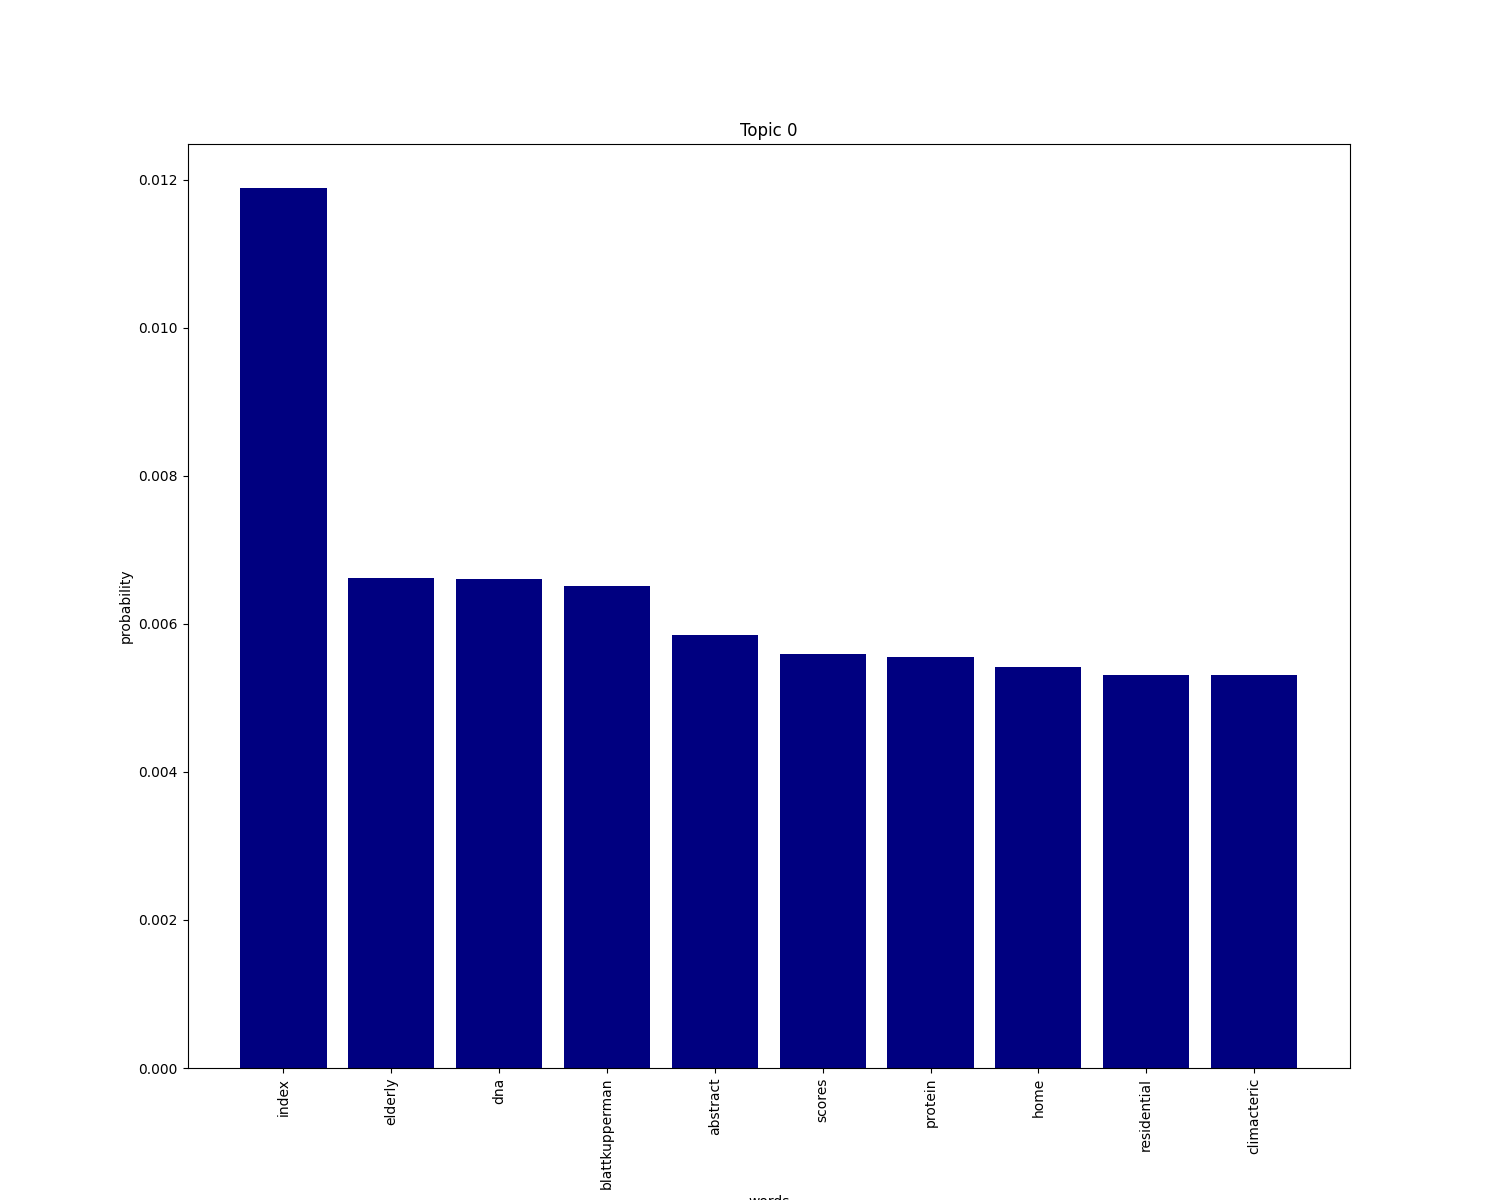
\includegraphics[width=7cm]{images/plots/test_5_no_stopwords_dataset_2/topic_0.png}
		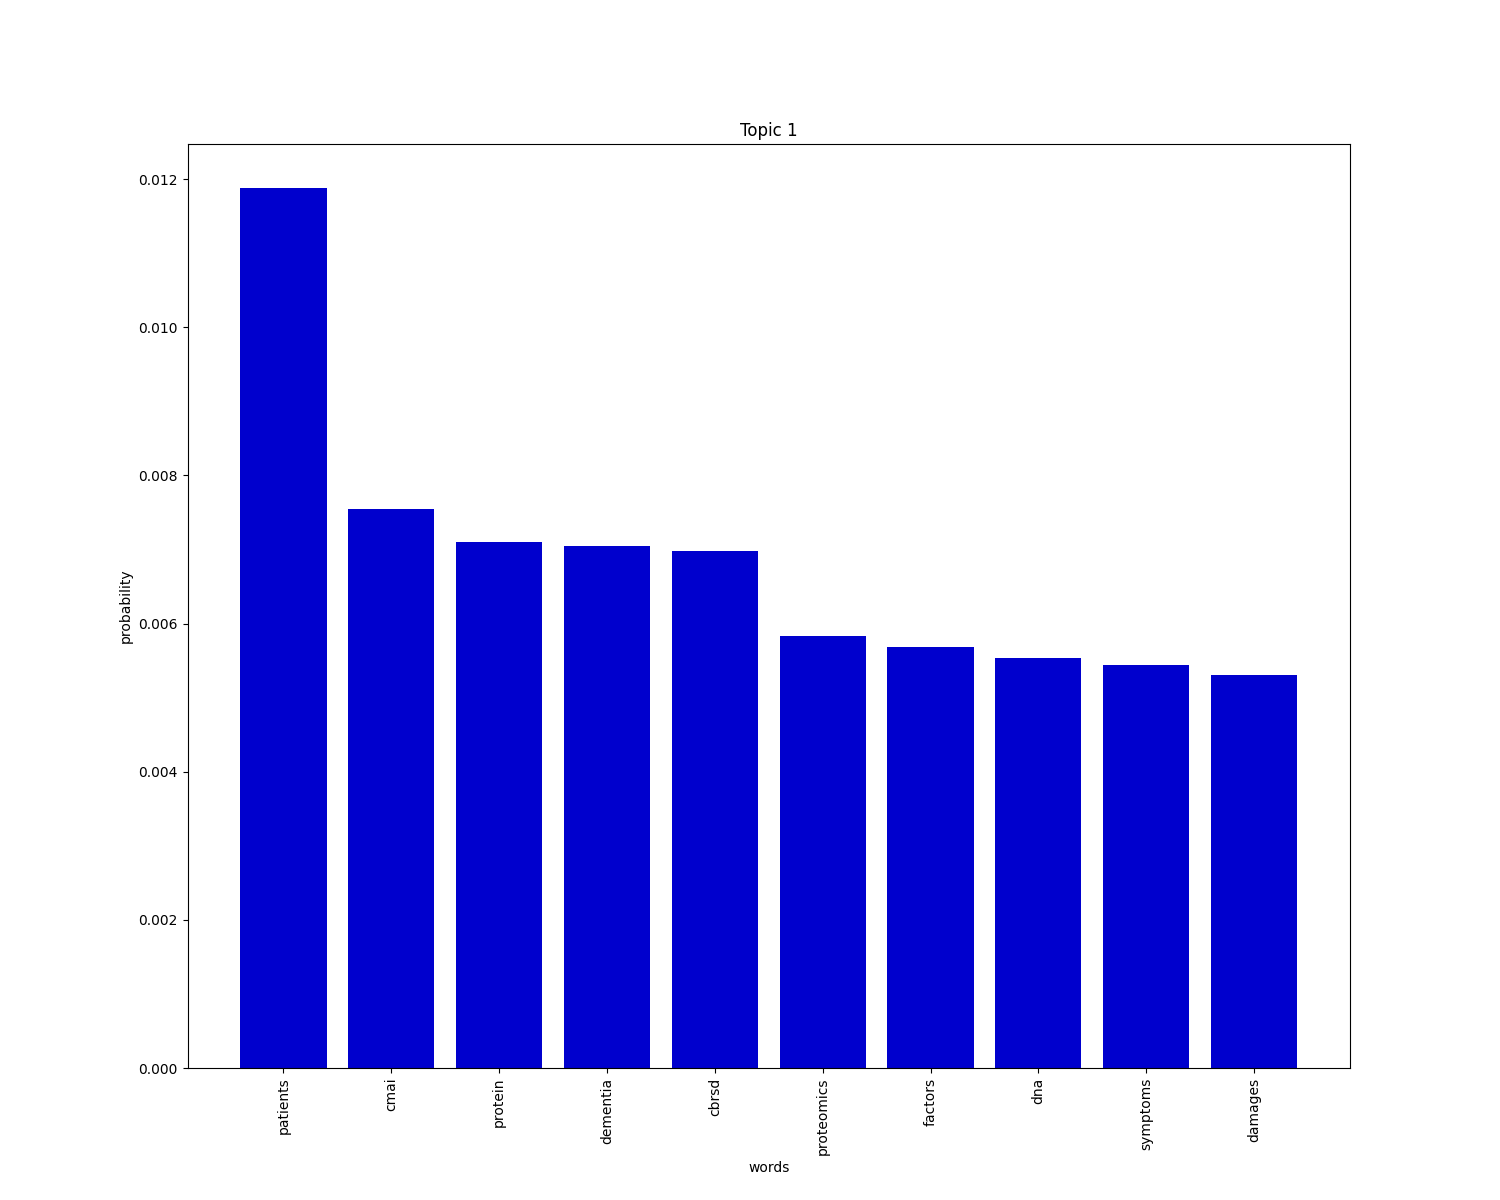
\includegraphics[width=7cm]{images/plots/test_5_no_stopwords_dataset_2/topic_1.png}
		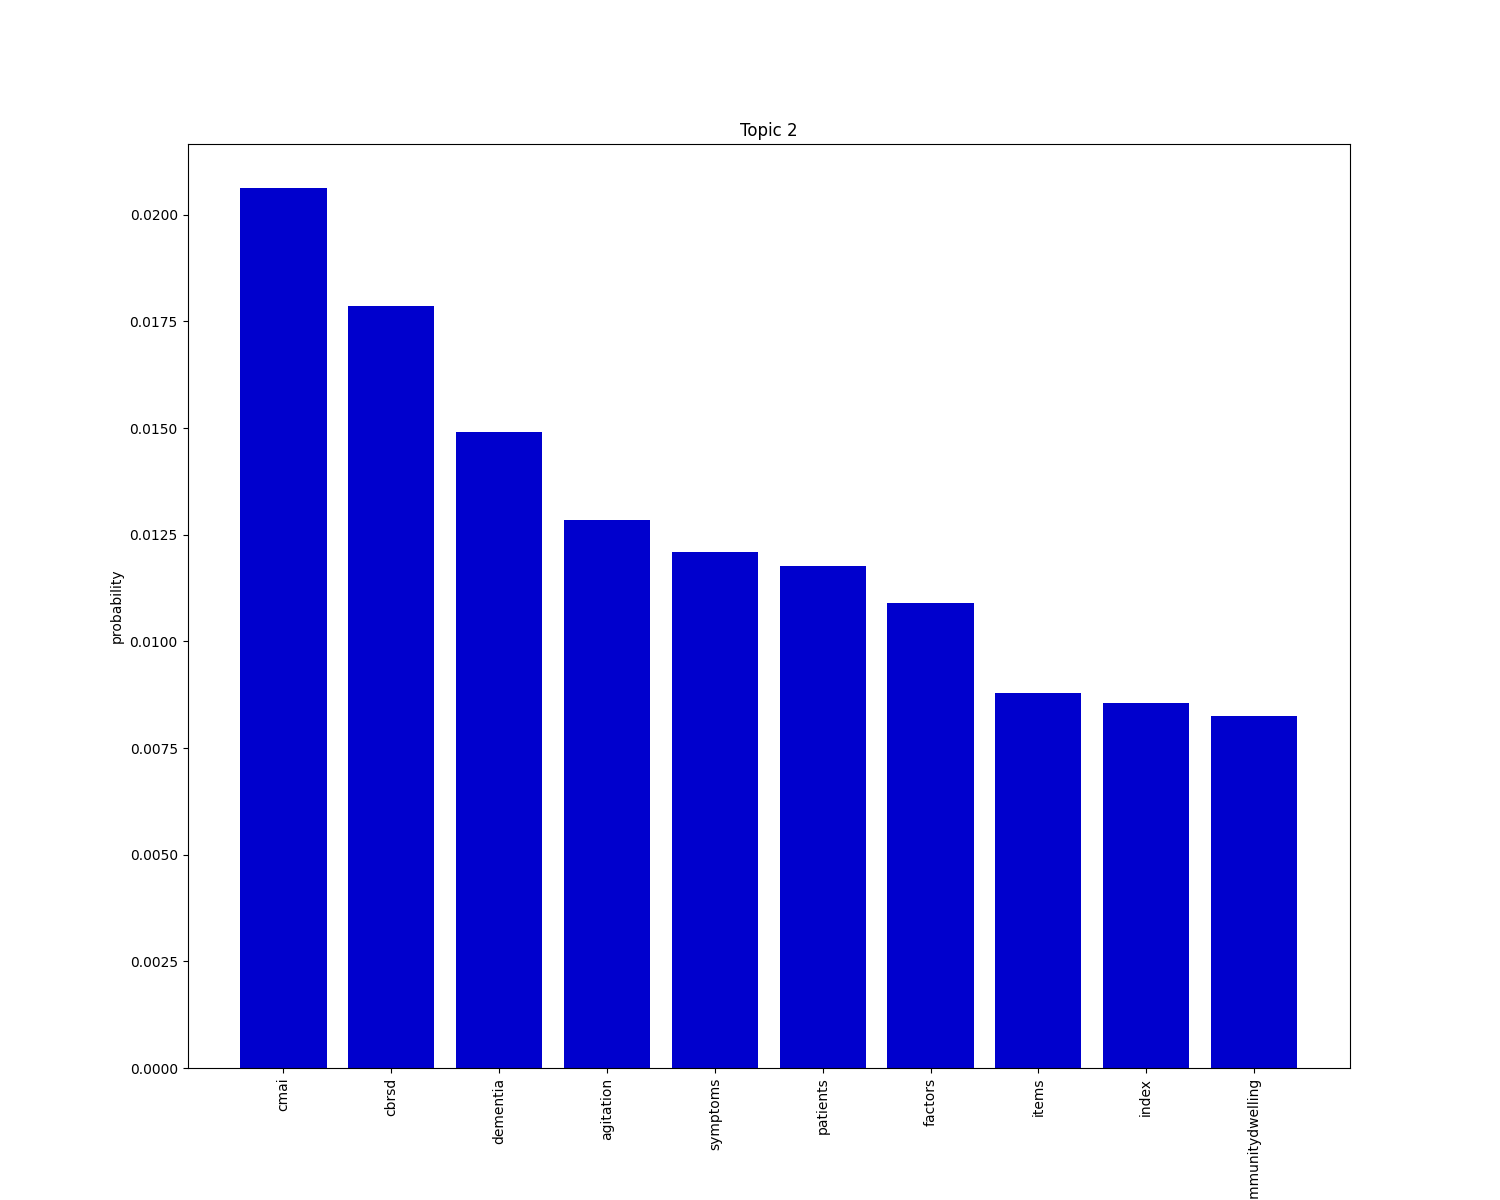
\includegraphics[width=7cm]{images/plots/test_5_no_stopwords_dataset_2/topic_2.png}
		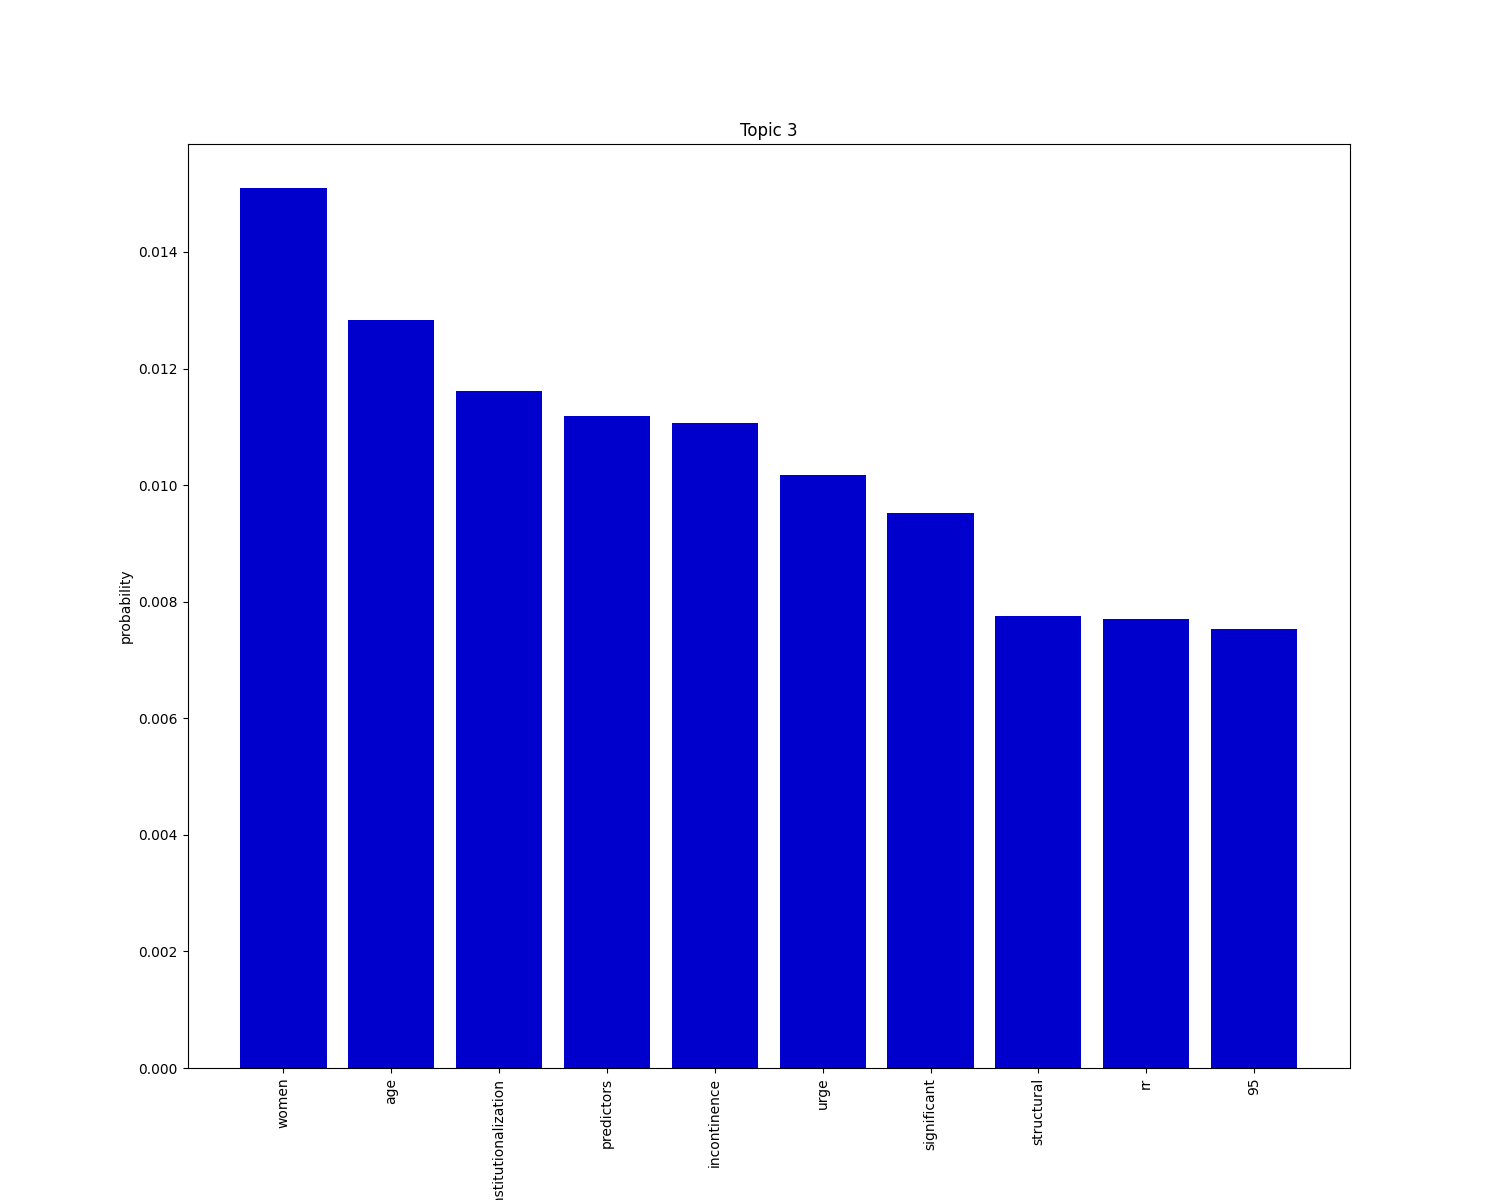
\includegraphics[width=7cm]{images/plots/test_5_no_stopwords_dataset_2/topic_3.png}
	\end{figure}
		
	
\begin{figure}[H]
	\centering
	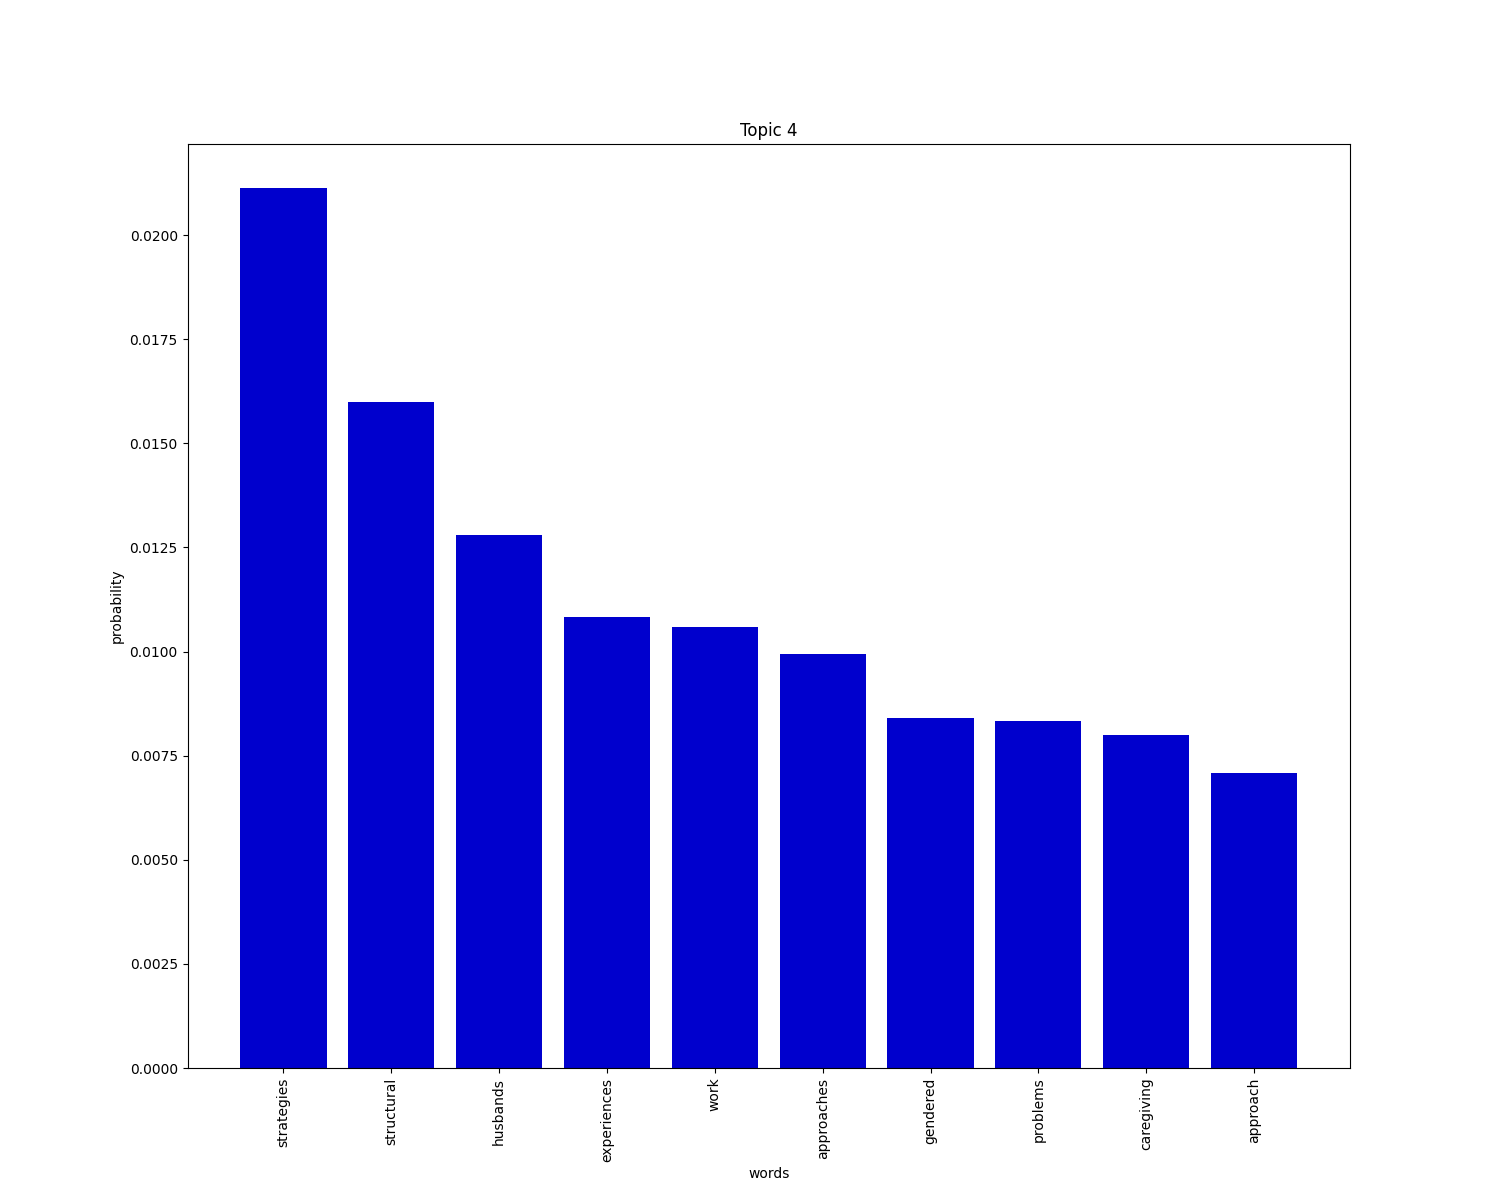
\includegraphics[width=7cm]{images/plots/test_5_no_stopwords_dataset_2/topic_4.png}
	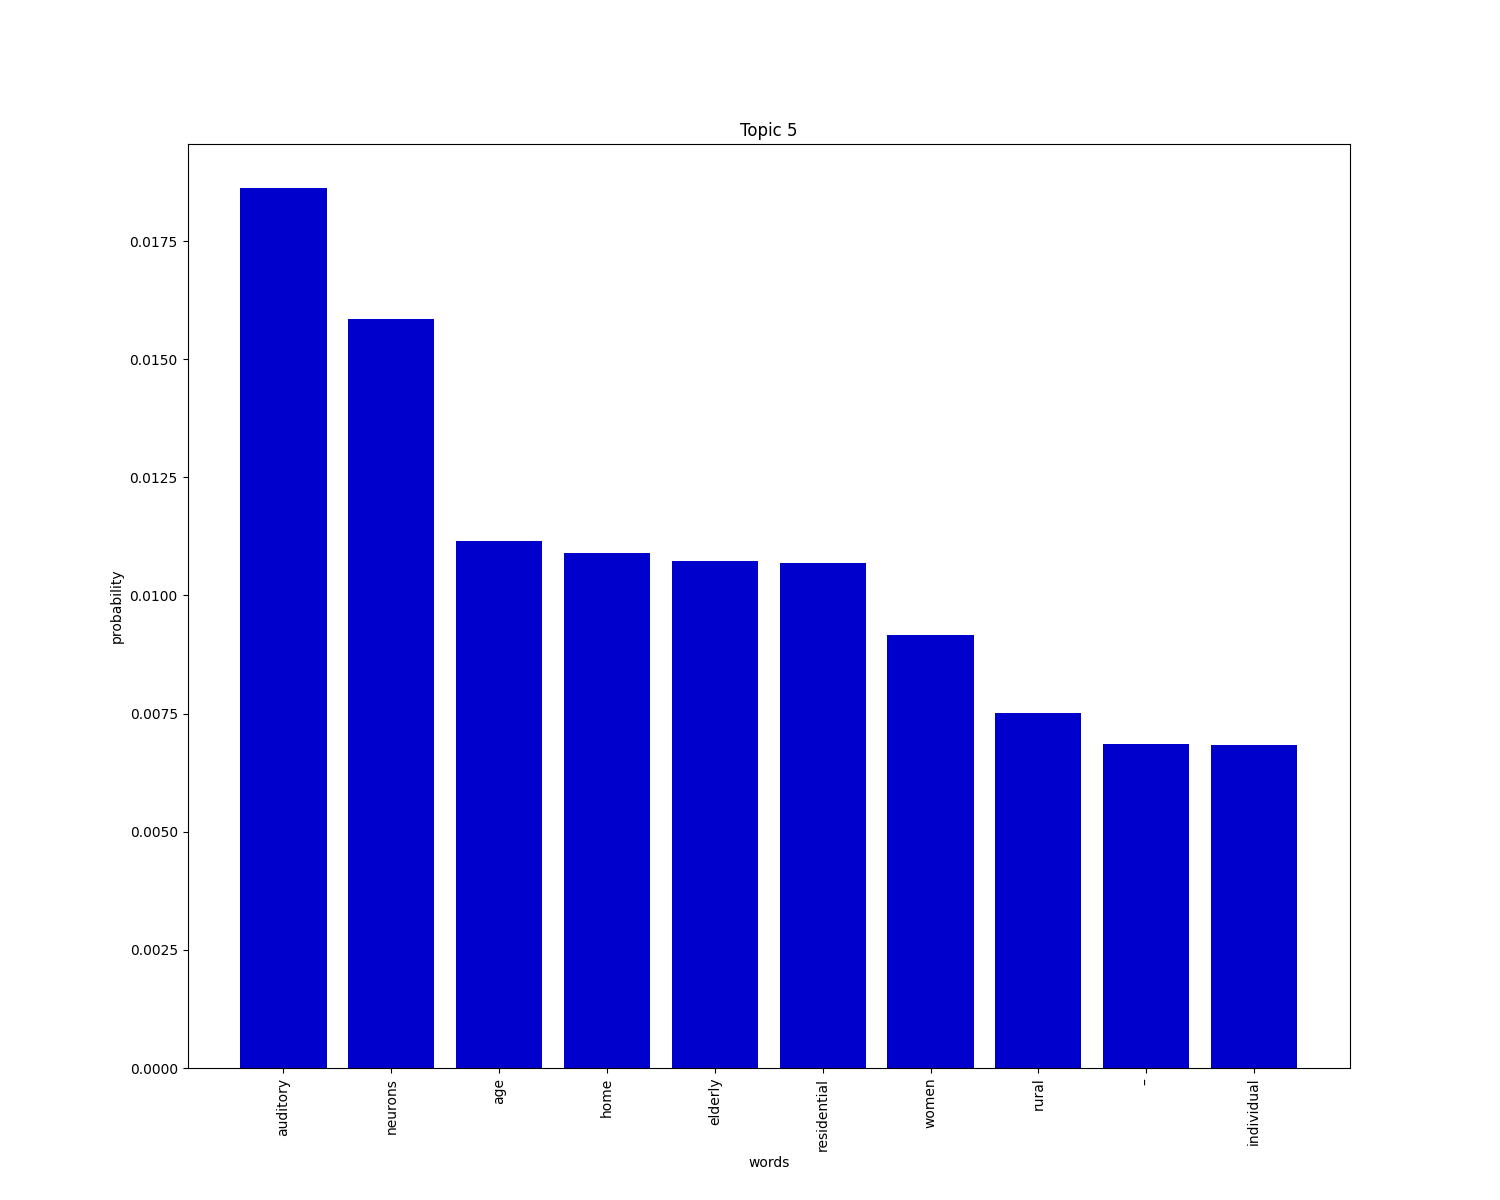
\includegraphics[width=7cm]{images/plots/test_5_no_stopwords_dataset_2/topic_5.png}
		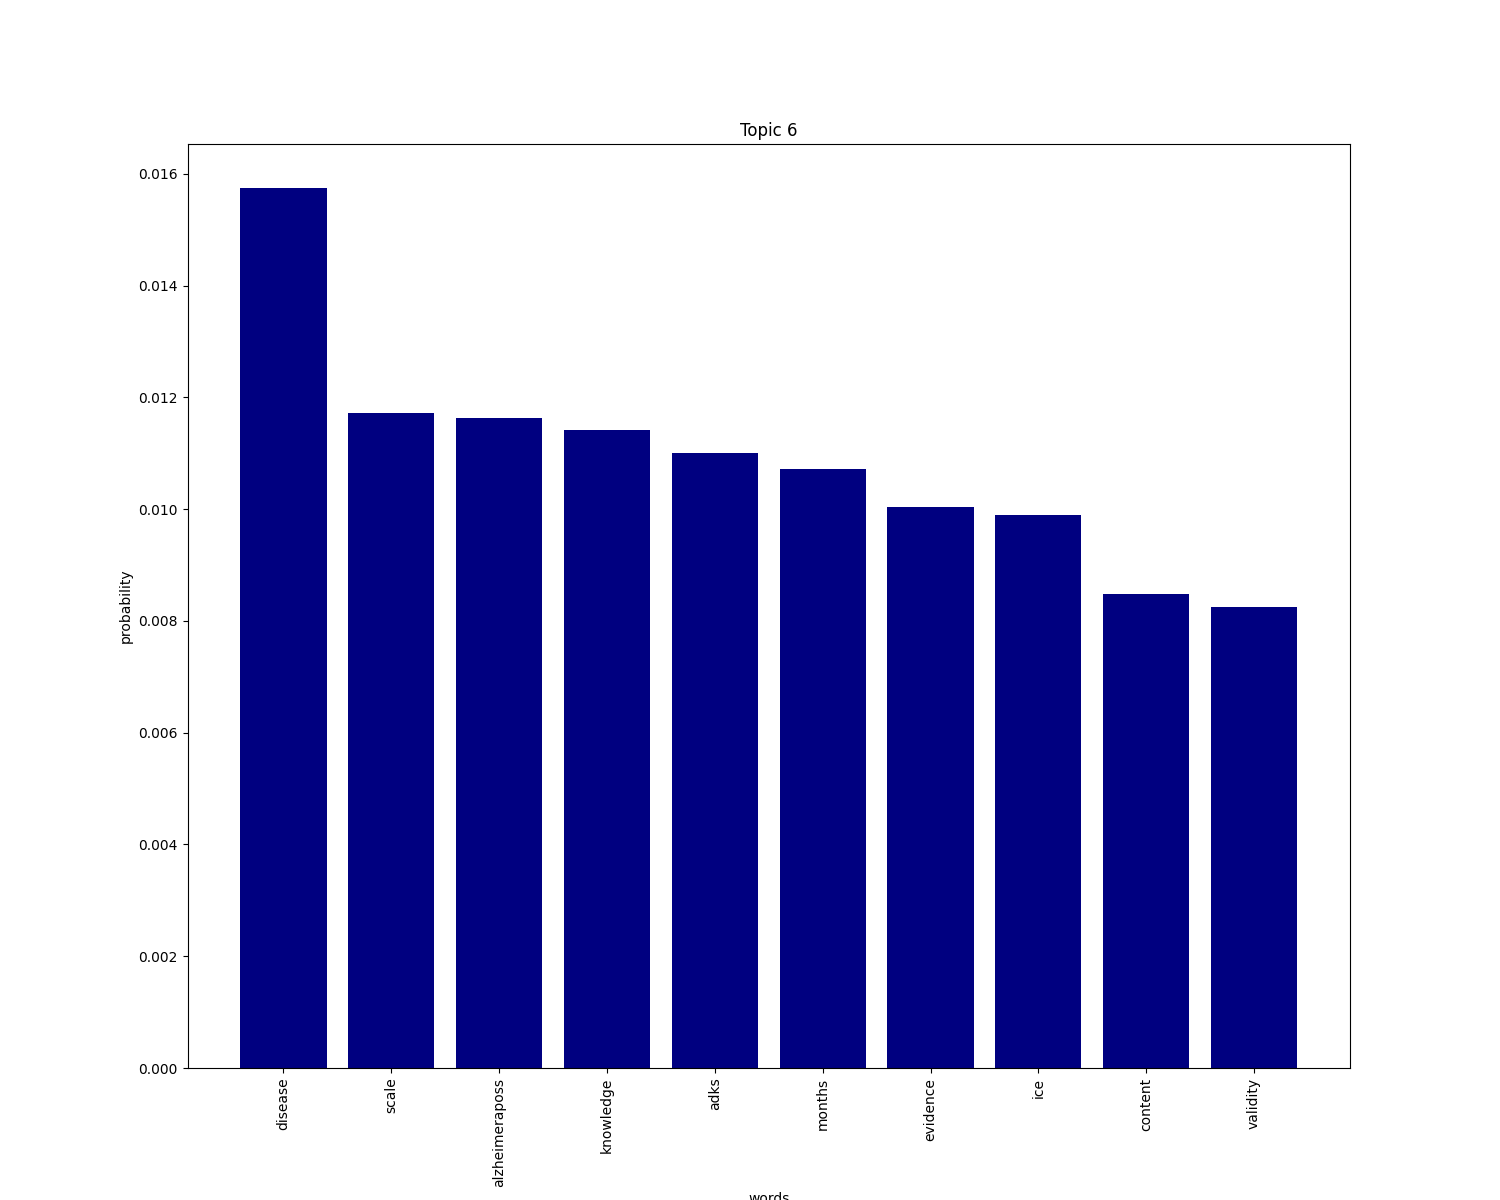
\includegraphics[width=7cm]{images/plots/test_5_no_stopwords_dataset_2/topic_6.png}
		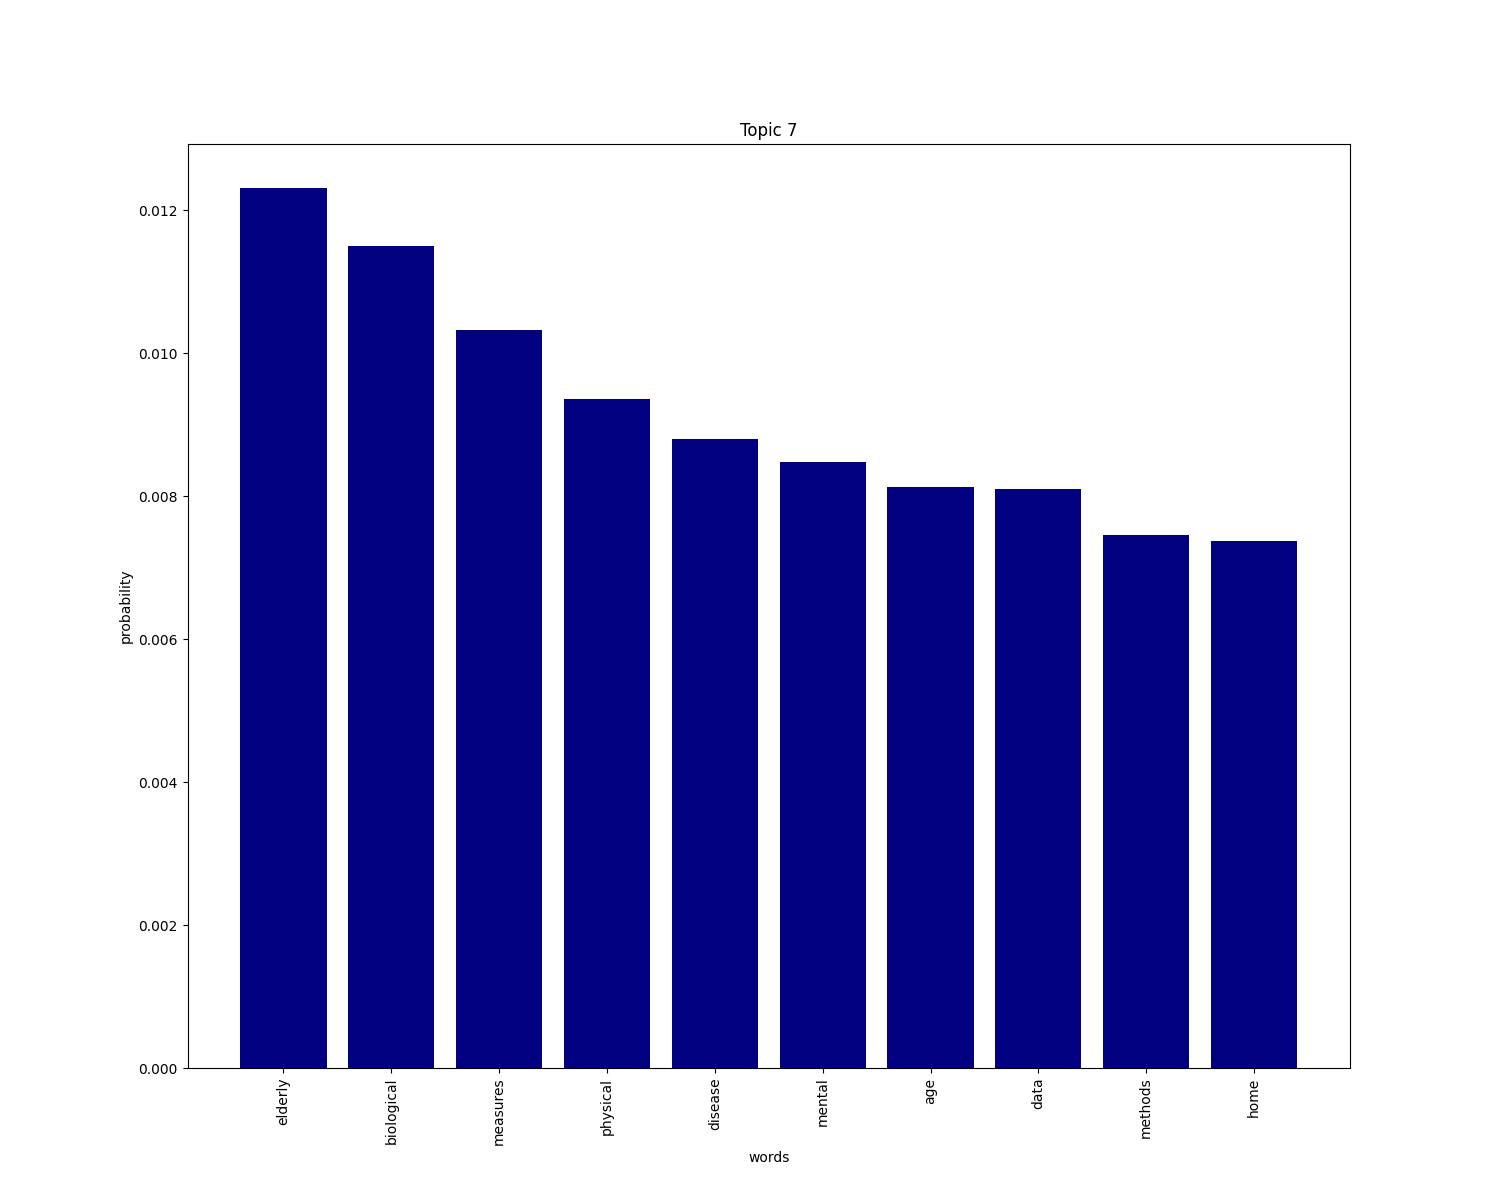
\includegraphics[width=7cm]{images/plots/test_5_no_stopwords_dataset_2/topic_7.png}	
	\caption{Topic description for test 5 of dataset TokenVieuxN after removing stopwords.}
\end{figure}
	
	We observe a coherence value of 0.50 and a perplexity value of -7.70. When juxtaposed with the performance of the model without stopwords on the previous dataset, it's possible to notice that the perplexity slightly increased and the coherence decreased. This comparative analysis suggests that the Latent Dirichlet Allocation (LDA) model, configured with 10 topics, provides a better fit for the data derived from the 'TokenVieuxM' dataset.
	
	\subsection{Optimal number of topics for the document collection TokenVieuxN.txt}
	
	As we can observe in the following plots associated with the current dataset, we find an analogous situation to the one encountered with the previous dataset: there is no discernible elbow. We will employ the same approach as previously outlined and use the composite metric to find the optimal number of topics for the LDA model.
	
		\begin{figure}[H]
		\centering
		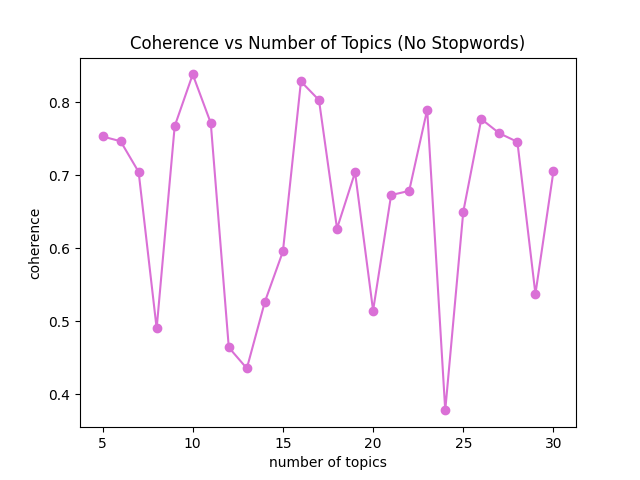
\includegraphics[width=7cm]{images/coherence_no_stopwords_diff_n_topics_2}
		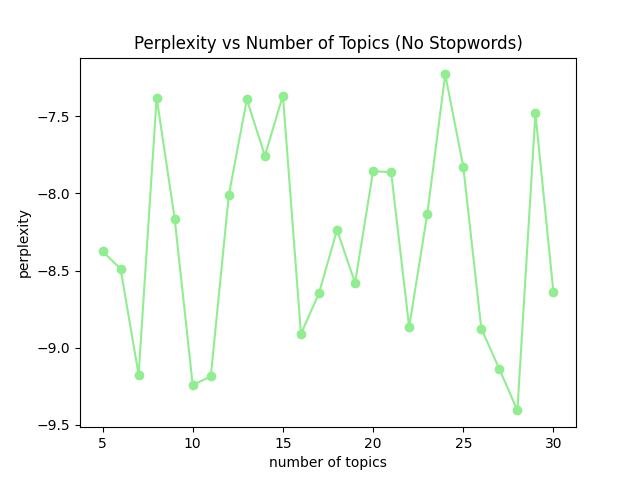
\includegraphics[width=7cm]{images/perplexity_no_stopwords_diff_n_topics_2}
	\caption{Coherence and perplexity values of the model for each number of topic $k \in [5, 30]$ , in dataset TokenVieuxN.}
\end{figure}
	
	The optimal number of topics would be 23.
	
\section{Most typical documents for topics}
To identify the most typical document for each topic we employed the \textit{get\_document\_topics} method provided by the \textit{LdaModel} class. This method returns a list of tuples, each containing the topic ID and the probability of that topic for a given document. 

The subsequent table presents the results derived from the document collection TokenVieuxM.txt. It is observable that the maximum probability value is 0.99302, corresponding to Document 5 that is associated with Topic 8. Conversely, the minimum probability value is 0.98846, attributed to Document 1 that is linked to Topic 4. The relatively minor disparity between the maximum and minimum values suggests that the model maintains a relatively uniform level of confidence across these documents.

\begin{figure}[H]
	\centering
	\begin{tabular}{|c|c|c|}
		\hline \textbf{Document} & \textbf{Topic ID} & \textbf{Topic Probability}  \\  
		\hline \textbf{1} & 4 & 0.98846 \\
		\hline \textbf{2} & 3 & 0.99099 \\
		\hline \textbf{3} & 1 & 0.98928 \\
		\hline \textbf{4} & 9 & 0.99262 \\
		\hline \textbf{5} & 8 & 0.99302 \\
		\hline
	\end{tabular}
	\caption{Most typical documents for topics in dataset TokenVieuxM.}
\end{figure}

The findings from the document collection TokenVieuxM.txt, as presented in the following table, demonstrate that document 6 pertaining to Topic 4 exhibits the highest probability value of 0.99451, whereas Document 7, also associated with Topic 4 exhibits the lowest probability value of 0.34179. This notable disparity between the highest and lowest probability values suggests that the model's level of confidence varies significantly when considering these specific documents.


\begin{figure}[H]
	\centering
	\begin{tabular}{|c|c|c|}
		\hline \textbf{Document} & \textbf{Topic ID} & \textbf{Topic Probability}  \\  
		\hline \textbf{1} & 9 & 0.98846 \\
		\hline \textbf{2} & 5 & 0.99099\\
		\hline \textbf{3} & 9 & 0.98928 \\
		\hline \textbf{4} & 7 & 0.99262 \\
		\hline \textbf{5} & 6 & 0.99302 \\
		\hline \textbf{6} & 4  & 0.99451 \\
		\hline \textbf{7} & 4 & 0.34179 \\
		\hline \textbf{8} & 7 & 0.98448 \\
		\hline \textbf{9} & 3 & 0.98815 \\
		\hline \textbf{10} & 1 & 0.98915 \\
		\hline
	\end{tabular}
	\caption{Most typical documents for topics in dataset TokenVieuxN.}
\end{figure}

\section{Code modifications, tests and plots}

The script utilized for this analysis, named \textit{CoherenceTestIwor.py}, is structured into three primary functions: \textit{read()}, \textit{parse()}, and \textit{lda()}. The \textit{read()} function is tasked with loading the specified dataset. The \textit{parse()} function processes the loaded dataset by eliminating unnecessary symbols and preparing the data for the LDA model. The \textit{lda()} function initializes an LDA model using the \textit{Gensim} library, taking the parsed dataset and the desired number of topics as inputs. This function also computes the coherence and perplexity of the model.

Furthermore, to complement the study, three additional scripts were developed: \textit{CoherenceTestIworStopwords.py} for conducting tests excluding stopwords, \textit{CoherenceTestIworStopwordsTypicalDocument.py} for identifying the most representative document for each topic, and \textit{Plot.py} for generating essential charts. The second script includes a function called \textit{document\_topics()} that initializes an LDA model and utilizes the \textit{get\_document\_topics()} method from the LdaModel class to determine the most representative documents for each topic. All of these scripts can be found within the \textit{src} folder.

Moreover, all the tests conducted during the analysis were saved in the \textit{test} folder. This folder is organized into two subfolders, each representing a distinct collection.

\begin{thebibliography}
	a
	\bibitem{1} Ali Daud, Juanzi Li, Lizhu Zhou, and Faqir Muhammad. \emph{Knowledge discovery through
	directed probabilistic topic models: a survey. Frontiers of Computer Science in China}, 4(2):280–
	301, June 2010.
	\bibitem{2} Thomas L. Griffiths and Mark Steyvers. \emph{Finding scientific topics}. Proceedings of the National
	Academy of Sciences, 101(suppl\_1):5228–5235, April 2004.
	\bibitem{3} Jean-Charles Lamirel, Yue Chen, Pascal Cuxac, Shadi Al Shehabi, Nicolas Dugué, and Zeyuan
	Liu. \emph{An overview of the history of Science of Science in China based on the use of bibliographic
	and citation data: a new method of analysis based on clustering with feature maximization
	and contrast graphs}. Scientometrics, 125(3):2971–2999, December 2020.
	\bibitem{4} David M Blei. \emph{Latent Dirichlet Allocation}. Journal of Machine Learning Research. 993-1022. January 2003.
\end{thebibliography}
\end{document}


